\section{Unobserved Auction Heterogeneity}\label{sec:15-uh}

Objects sold in different auctions differ, and bidders usually know more about the differences than
the econometrician does. A paving contractor visits the site and sees the curvature of the road and
the state of the surface. A used-car dealer inspects each car for rust and dents. Such features
shift every bidder's value in the same direction, and they are common knowledge among the bidders.
When the econometrician cannot condition on them, the methods of \cref{sec:15-gpv,sec:15-apv}
attribute their effect to private information. This section shows what goes wrong and develops
three remedies. They are deconvolution with several bids per auction, parametric mixtures, and
control functions built from the seller's reserve price.

\subsection{The problem}\label{sec:15-uh-problem}

Let $\omega_t$ be a scalar characteristic of auction $t$ that all bidders, and the seller, observe
but the econometrician does not. We call $\omega_t$ \emph{unobserved auction heterogeneity}. The two
workhorse specifications are additive and multiplicative,
\begin{equation}\label{eq:15-uh-values}
V_{it}=\omega_t+A_{it}\qquad\text{or}\qquad V_{it}=\omega_tA_{it},
\end{equation}
where $A_{it}$ is bidder $i$'s \emph{idiosyncratic private component}. In procurement we write
costs as $C_{it}=\omega_tA_{it}$ in the same way.

\begin{assumption}[Unobserved auction heterogeneity]\label{ass:15-uh}
(i) In each auction, $\omega_t,A_{1t},\dots,A_{nt}$ are mutually independent, $\omega_t\sim F_\omega$
and $A_{it}\sim F_{A_i}$, and auctions are independent. (ii) Each bidder observes $\omega_t$, its own
$A_{it}$ and the number of bidders $n_t$. The econometrician observes bids and $n_t$ but neither
$\omega_t$ nor $A_{it}$. (iii) For each $\omega_t$, bidders play the unique equilibrium of the game
with that common component.
\end{assumption}

The same equation \eqref{eq:15-uh-values} with bidders who observe only their own sums $V_{it}$
describes a \emph{conditionally independent private values} model. It is a special case of affiliated
private values when the densities $f_{A_i}$ are log-concave \citep[Section 6.1.2]{AtheyHaile2007}.
The two models differ only in what bidders know. With unobserved heterogeneity, bidder $i$ knows
that its rivals' values are centered on $\omega_t$, so its uncertainty about the competition is the
dispersion of the $A_{jt}$ alone.

The information that is common knowledge among the bidders in auction $t$ is the pair
$(Z_t,\omega_t)$ of observed covariates and unobserved heterogeneity. In a private values first-price
auction, the first-order condition \eqref{eq:14-apv-foc} holds conditionally on it
\citep[Section 6.1.2]{AtheyHaile2007},
\begin{equation}\label{eq:15-uh-foc}
v_{it}=b_{it}+\frac{G_{M\mid B}(b_{it}\mid b_{it};n_t,Z_t,\omega_t)}{g_{M\mid B}(b_{it}\mid b_{it};n_t,Z_t,\omega_t)} .
\end{equation}
An econometrician who does not observe $\omega_t$ cannot estimate the conditional distribution that
enters the markdown. Pooling auctions with different $\omega_t$ replaces it with a mixture over
$\omega_t$. The markdown is a nonlinear function of $\omega_t$, so even its average is not identified without further
structure \citep[Section 6.1.2, citing \citealp{HendricksPinksePorter2003}]{AtheyHaile2007}.

\citet[Section 6.1.2]{AtheyHaile2007} separate three questions.
\begin{enumerate}[label=(\roman*)]
\item \emph{Can unobserved heterogeneity be told apart from other sources of correlated bids?} In an
ascending auction a bidder drops out at its value whether or not it observes $\omega_t$. Unobserved
heterogeneity is then observationally equivalent to correlated private values. In a first-price
auction, any bid distribution that satisfies the conditions of \cref{thm:15-ah-rational} can be
rationalized by affiliated private values without heterogeneity. The choice between the two models
must rest on institutional knowledge.
\item \emph{Is the joint law of $(\omega,A_1,\dots,A_n)$ identified under heterogeneity?} In
first-price auctions it is, under separability and independence, as we show below. In ascending
auctions it requires additional variation, such as bidder covariates (\cref{thm:15-ah5}).
\item \emph{Which primitives does a question need?} In ascending and second-price auctions bidding is
in dominant strategies, so the joint law $F_{\bm V}$ of values answers every counterfactual. First-price
counterfactuals depend on beliefs, and beliefs vary with $\omega_t$. They require the joint law of the
components, $F_{\omega,\bm A}$. The joint law of values $F_{\bm V}$ is not enough.
\end{enumerate}

Ignoring $\omega_t$ has a predictable effect on first-price estimates. Bids from auctions with high
and low $\omega_t$ are pooled, so the estimated bid distribution is too dispersed. Each bidder appears
to face a field of rivals that is more spread out than the one it faces in fact. The estimated
markdown $\frac{G(b)}{(n-1)g(b)}$ is then too large, and so are estimated markups and the estimated
dispersion of values \citep[pp.~294--295]{Krasnokutskaya2011}.

\begin{example}[Pooling bids across heterogeneous auctions]\label{ex:15-uh-uniform}
Let $n=4$, $V_{it}=\omega_tA_{it}$, $A_{it}\sim U[1,2]$ and $\ln\omega_t\sim N(0,0.3^2)$. At
$\omega=1$ the game is a symmetric IPV auction with $F_A(a)=a-1$ on $[1,2]$. The Riley-Samuelson bid
\eqref{eq:14-rs-bid} with no reserve price is
\[
\alpha(a)=a-\frac{\int_1^a(t-1)^3\,dt}{(a-1)^3}=a-\frac{a-1}{4}=\frac{3a+1}{4}.
\]
By \cref{lem:15-separability}(b) below, the bid at $\omega$ is $\beta(v;\omega)=\omega\,\alpha\big(\frac{v}{\omega}\big)
=\frac{3v+\omega}{4}$. The markdown relative to value,
$\frac{v-\beta(v;\omega)}{v}=\frac{a-\alpha(a)}{a}=\frac{a-1}{4a}$, does not depend on $\omega$. Its
average is
\[
\E\Big[\frac{A-1}{4A}\Big]=\frac{1}{4}\Big(1-\E\Big[\frac{1}{A}\Big]\Big)=\frac{1}{4}\big(1-\ln 2\big)\approx0.077 .
\]
We simulated 200 samples of $T=500$ such auctions and applied the GPV estimator of \cref{sec:15-gpv} to
the pooled bids (seed 15701, script \texttt{uh\_bias.py}). The median estimate of the average markdown
is $0.184$, with 5th and 95th percentiles of $0.174$ and $0.193$ across samples. The estimated inverse
bid function in \cref{fig:15-uh-bias}(a) has slope $1.47$ over the central bids, against the true
slope $\frac{4}{3}$. The estimated value density in panel (b) roughly tracks the marginal density of
$V=\omega A$ but is more spread out. Computed over the plotted range $[0.4,3.6]$, its variance is
$0.376$ against $0.300$ for $V$. On the full support the exact variance of $V$ is
$e^{0.18}\cdot\frac{7}{3}-\big(1.5e^{0.045}\big)^2=0.332$. The estimated density has a long upper tail,
from bids where $\hat g$ is small, which raises its full-support variance to about $1.4$. The
interquartile range is less sensitive to that tail. It is $0.97$ for the pseudo-values (median across
samples) against $0.73$ for $V$. Both are far more dispersed than the distribution $F_A$, with
interquartile range $0.5$, that each bidder faces once it has seen $\omega_t$.
\end{example}

\begin{figure}[htbp]
\centering
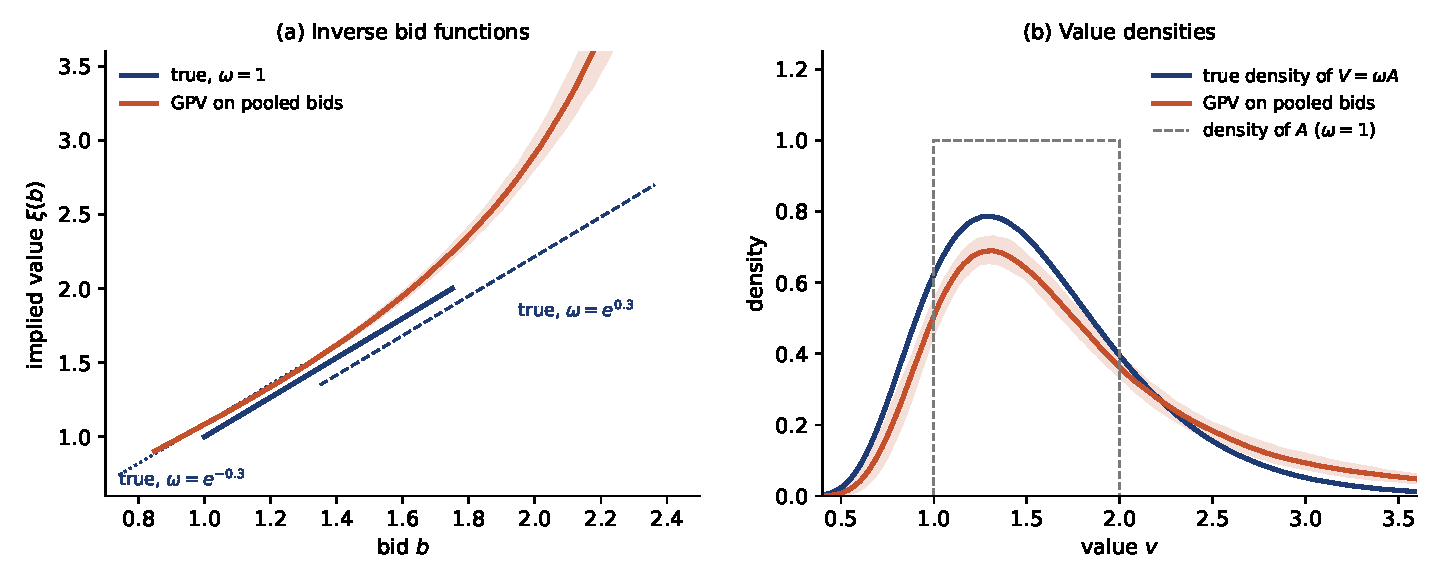
\includegraphics[width=\textwidth]{figures/ch15/uh_bias.pdf}
\caption{GPV applied to bids pooled across auctions with unobserved heterogeneity (our simulation,
seed 15701). Design of \cref{ex:15-uh-uniform}: $n=4$, $V=\omega A$, $A\sim U[1,2]$,
$\ln\omega\sim N(0,0.3^2)$, $T=500$ auctions, 200 samples. Panel (a): true inverse bid functions at
three values of $\omega$ and the median GPV estimate from pooled bids with a 5--95 percent band. Panel
(b): the true marginal density of $V$, the density of $A$ that bidders face at $\omega=1$, and the
median GPV estimate with its band. The true average markdown is $0.077$ and the median estimate is
$0.184$.}
\label{fig:15-uh-bias}
\end{figure}

\subsection{Separability and homogenization}\label{sec:15-uh-sep}

Equilibrium bidding inherits the additive or multiplicative structure of values. This property drives
every method in this section.

\begin{lemma}[Separability, after \citealp{AtheyHaile2007}, eqs. (6.4)--(6.5), and \citealp{Krasnokutskaya2011}, Proposition 1]\label{lem:15-separability}
Let \cref{ass:15-uh} hold with no binding reserve price. Let $(\alpha_1,\dots,\alpha_n)$ be the
equilibrium bid functions of the \emph{normalized game}, the game with $\omega=0$ in the additive case
and $\omega=1$ in the multiplicative case.
\begin{enumerate}[label=(\alph*)]
\item In a first-price auction with additive values, $\beta_i(v;\omega)=\omega+\alpha_i(v-\omega)$.
\item In a first-price procurement auction with multiplicative costs $C_i=\omega A_i$,
$\beta_i(c;\omega)=\omega\,\alpha_i\big(\frac{c}{\omega}\big)$. In a first-price auction with
multiplicative values $V_i=\omega A_i$, likewise $\beta_i(v;\omega)=\omega\,\alpha_i\big(\frac{v}{\omega}\big)$.
\item The \emph{homogenized bids} $B^0_{it}=B_{it}-\omega_t$ in case (a) and $B^0_{it}=\frac{B_{it}}{\omega_t}$
in case (b) equal $\alpha_i(A_{it})$. They are independent of $\omega_t$ and of each other, and they
have the bid distributions of the normalized game.
\end{enumerate}
\end{lemma}

\begin{proof}
We prove (b), the case used in the application below. Suppose bidders $j\neq i$ use
$\beta_j(c;\omega)=\omega\,\alpha_j\big(\frac{c}{\omega}\big)$ in the game with common component
$\omega$. A bidder with cost $C_j=\omega A_j$ then bids $\omega\,\alpha_j(A_j)$. Bidder $i$ wins with
bid $b$ when every rival bids more,
\[
\Pr\big(\text{$i$ wins}\mid b\big)=\Pr\big(\omega\,\alpha_j(A_j)>b\ \ \forall j\neq i\big)
=\Pr\Big(\alpha_j(A_j)>\frac{b}{\omega}\ \ \forall j\neq i\Big)\equiv P^0_i\Big(\frac{b}{\omega}\Big),
\]
where $P^0_i(a')$ is bidder $i$'s probability of winning with bid $a'$ in the normalized game. A bidder
with cost $c=\omega a$ who bids $b$ earns
\[
(b-\omega a)\,P^0_i\Big(\frac{b}{\omega}\Big)=\omega\Big(\frac{b}{\omega}-a\Big)P^0_i\Big(\frac{b}{\omega}\Big).
\]
Choosing $b$ is the same as choosing $a'=\frac{b}{\omega}$ to maximize $(a'-a)P^0_i(a')$. That is
bidder $i$'s problem in the normalized game, and its solution is $a'=\alpha_i(a)$. Hence the best
response is $b=\omega\,\alpha_i(a)=\omega\,\alpha_i\big(\frac{c}{\omega}\big)$, and the profile is an
equilibrium of the game with $\omega$. By \cref{ass:15-uh}(iii) it is the equilibrium. The sale
auction with $V_i=\omega A_i$ follows word for word, with $(v-b)$ in place of $(b-c)$ and win
probabilities $\Pr\big(\omega\,\alpha_j(A_j)<b\ \forall j\neq i\big)$. Part (a)
follows from the same argument with $b-\omega$ in place of $\frac{b}{\omega}$ and $(v-\omega)$ in place
of $a$. For (c), $B^0_{it}=\alpha_i(A_{it})$ is a function of $A_{it}$ alone, and the $A_{it}$ are
independent of $\omega_t$ and of each other.
\end{proof}

The argument needs the whole game to scale with $\omega$. A reserve price that does not move with
$\omega$ breaks it, which is one reason the application below relies on a nonbinding reserve. If the
number of bidders responds to $\omega_t$ through entry, part (c) holds only conditional on $n_t$, and
$n_t$ itself carries information about $\omega_t$.

\casehead{Homogenization with observed covariates}
Separability is useful even when all heterogeneity is observed. \Cref{sec:15-covariates} homogenized
transaction prices in ascending auctions, where bids equal values. \citet[Section 6.1.1]{AtheyHaile2007},
following \citet{HaileHongShum2003}, carry the idea over to first-price bids. Suppose, as in
\cref{thm:15-ah3}(ii), that $V_{it}=g_0(Z_t)+A_{it}$ with $A_{it}$ independent of $Z_t$ and the
normalization $g_0(z_0)=0$. \Cref{lem:15-separability}(a) with $\omega_t=g_0(Z_t)$ gives
$\beta_i(v;n,z)=g_0(z)+\beta_i\big(v-g_0(z);n,z_0\big)$. Bids therefore satisfy the regression
\begin{equation}\label{eq:15-homog-reg}
b_{it}=\kappa(n_t)+g_0(z_t)+\varepsilon_{it},\qquad
\varepsilon_{it}=\beta_i(V_{it}-g_0(z_t);n_t,z_0)-\kappa(n_t),\qquad \E[\varepsilon_{it}\mid z_t,n_t]=0,
\end{equation}
where $\kappa(n)$ is an intercept for $n$-bidder auctions, as in \cref{sec:15-covariates}. Ordinary least
squares on all bids estimates $g_0$. The homogenized bids $\hat b_{it}=b_{it}-\hat g_0(z_t)$ estimate
the bids that would have been placed at $z_0$. The GPV estimator applied to them, separately for each $n$,
recovers $F_V(\cdot;z_0)$, and then $F_V(v;z)=F_V\big(v-g_0(z);z_0\big)$ for every $z$. The first stage
uses all $\sum_nnT_n$ bids, so a flexible parametric $g_0$ converges at the parametric rate. As in the
ascending case, it leaves the nonparametric asymptotics of the second stage unchanged. The multiplicative
case works the same way in logs. \citet[eqs. (6.7)--(6.9)]{AtheyHaile2007} also describe sieve and finite-mixture
specifications of the bid distribution. These let covariates affect bids more flexibly, at the cost
of a priori structure, and covariate effects are then recovered only indirectly.

\casehead{Why unobserved heterogeneity needs more}
With $\omega_t$ unobserved, the analogue of \eqref{eq:15-homog-reg} is
$\ln b_{it}=\ln\omega_t+\ln B^0_{it}$. The term $\ln\omega_t$ is an auction fixed effect that cannot be
subtracted. The structure nevertheless suggests a remedy. Two bids from the same auction are two
noisy measurements of the same $\ln\omega_t$, with independent errors $\ln B^0_{it}$. This is the
repeated-measurement problem of the measurement-error literature \citep{LiVuong1998}, and
deconvolution solves it \citep[Section 6.1.2 and footnote 51]{AtheyHaile2007}.

\subsection{Identification by deconvolution: Krasnokutskaya (2011)}\label{sec:15-krasno}

\subsubsection{Question and model}

\citet{Krasnokutskaya2011} asks how much of the variation in contractors' costs is private
information, and how far IPV and APV estimators err when bidders share cost information that the
econometrician lacks. The answer matters for markups, for the efficiency of first-price
procurement, and for any policy evaluated with an estimated cost distribution. Her abstract states
that accounting for unobserved heterogeneity ``has important implications for the evaluation of the
distribution of rents, efficiency, and optimal auction design'' (p.~293). We cite the published
article by page. Some material appears only in the 2004 working paper \citep{Krasnokutskaya2004},
which we mark WP. Its application used a different sample and reported different headline numbers.
We give the published numbers and say where the WP figures differ.

There are $n$ bidders of two observable types, $n_1$ of type 1 and $n_2=n-n_1$ of type 2. Bidder
$i$'s cost of the project in auction $t$ is $C_{it}=\omega_tA_{it}$. The maintained assumptions
are the following (pp.~296--297).
\begin{enumerate}[label=(D\arabic*)]
\item $\omega_t,A_{1t},\dots,A_{nt}$ are mutually independent. $A_{it}$ has distribution $F_{k}$ for a
type-$k$ bidder, and the supports $[\underline\omega,\bar\omega]$ and $[\underline a,\bar a]$ lie in
$(0,\infty)$.
\item The densities $f_1,f_2$ are continuously differentiable and strictly positive on the interior
of the support.
\item $\E[A_{it}]=1$ for type-1 bidders.
\item The number of bidders is common knowledge, and there is no binding reserve price.
\end{enumerate}
(D1) is the identifying assumption. (D2) delivers existence and uniqueness of the equilibrium. (D3)
fixes the scale, since $(\omega,A)$ and $(c\,\omega,\frac{A}{c})$ produce the same costs. For each
$\omega$ the game is an asymmetric IPV procurement auction. Krasnokutskaya attributes the existence of a
unique equilibrium in strictly monotone, differentiable strategies to McAdams and others (p.~297). By
\cref{lem:15-separability}(b), $B_{it}=\omega_t\,\alpha_{k(i)}(A_{it})$, where $k(i)$ is bidder $i$'s
type. This is her Proposition 1, which she notes also holds for additive components (p.~298,
footnote 3).

Let $G^0_k$ and $g^0_k$ be the distribution and density of the homogenized bid $B^0=\alpha_k(A)$ of a
type-$k$ bidder, and write $-k$ for the other type. In the normalized game a type-$k$ bidder with cost
$a$ who bids $b^0$ wins with probability
$P^0_k(b^0)=\big(1-G^0_k(b^0)\big)^{n_k-1}\big(1-G^0_{-k}(b^0)\big)^{n_{-k}}$. Its first-order condition is
$P^0_k(b^0)+(b^0-a)P^{0\prime}_k(b^0)=0$, so that $a=b^0+\frac{P^0_k(b^0)}{P^{0\prime}_k(b^0)}$ with
\[
\frac{P^{0\prime}_k(b^0)}{P^0_k(b^0)}=-\frac{(n_k-1)\,g^0_k(b^0)}{1-G^0_k(b^0)}-\frac{n_{-k}\,g^0_{-k}(b^0)}{1-G^0_{-k}(b^0)} .
\]
Substituting gives the inverse bid function in terms of homogenized bid distributions (her eq. (1)
and condition (W6), pp.~298 and 302),
\begin{equation}\label{eq:15-krasno-inverse}
a=\xi_k(b^0)\equiv b^0-\frac{\big(1-G^0_k(b^0)\big)\big(1-G^0_{-k}(b^0)\big)}{(n_k-1)\,g^0_k(b^0)\big(1-G^0_{-k}(b^0)\big)+n_{-k}\,g^0_{-k}(b^0)\big(1-G^0_k(b^0)\big)} .
\end{equation}
This is the asymmetric procurement condition of \cref{sec:14-procurement}, applied to the normalized
game. It would identify $F_k$ immediately if homogenized bids were observed. They are not, because
$\omega_t$ is not.

\subsubsection{Kotlarski's lemma}

Deconvolution rests on a characterization result for sums of independent random variables. We write
$\mathrm i=\sqrt{-1}$ for the imaginary unit and $\varphi_Y(t)=\E\big[e^{\mathrm i tY}\big]$ for the
\emph{characteristic function} of a random variable $Y$ (\cref{app:math}).

\begin{lemma}[\citealp{Kotlarski1966}, and \citealp{AtheyHaile2007}, Lemma 6.1]\label{lem:15-kotlarski}
Let $Y_1,Y_2,Y_3$ be mutually independent random variables with finite means and characteristic
functions $\varphi_1,\varphi_2,\varphi_3$ that never vanish. Let $Q_1=Y_1+Y_3$ and $Q_2=Y_2+Y_3$, and let
$\Psi(t_1,t_2)=\E\big[e^{\mathrm i(t_1Q_1+t_2Q_2)}\big]$ be their joint characteristic function, with
partial derivative $\Psi_1$ in its first argument.
\begin{enumerate}[label=(\roman*)]
\item The joint distribution of $(Q_1,Q_2)$ determines the distributions of $Y_1,Y_2,Y_3$ up to
location.
\item Under the normalization $\E[Y_1]=0$,
\begin{equation}\label{eq:15-kotlarski}
\varphi_3(t)=\exp\Big(\int_0^t\frac{\Psi_1(0,u)}{\Psi(0,u)}\,du\Big),\qquad
\varphi_1(t)=\frac{\Psi(t,0)}{\varphi_3(t)},\qquad \varphi_2(t)=\frac{\Psi(0,t)}{\varphi_3(t)} .
\end{equation}
\end{enumerate}
\end{lemma}

\begin{proof}
\emph{Step 1.} By independence,
\[
\Psi(t_1,t_2)=\E\big[e^{\mathrm it_1Y_1}\,e^{\mathrm it_2Y_2}\,e^{\mathrm i(t_1+t_2)Y_3}\big]
=\varphi_1(t_1)\,\varphi_2(t_2)\,\varphi_3(t_1+t_2).
\]
\emph{Step 2.} Finite means make each $\varphi_j$ differentiable, with $\varphi_j'(0)=\mathrm i\,\E[Y_j]$.
Differentiating in $t_1$,
\[
\Psi_1(t_1,t_2)=\varphi_1'(t_1)\varphi_2(t_2)\varphi_3(t_1+t_2)+\varphi_1(t_1)\varphi_2(t_2)\varphi_3'(t_1+t_2).
\]
\emph{Step 3.} At $t_1=0$, use $\varphi_1(0)=1$ and $\varphi_1'(0)=\mathrm i\,\E[Y_1]=0$:
\[
\Psi_1(0,u)=\varphi_2(u)\,\varphi_3'(u),\qquad \Psi(0,u)=\varphi_2(u)\,\varphi_3(u).
\]
\emph{Step 4.} Since $\varphi_2(u)\neq0$, dividing gives
$\frac{\Psi_1(0,u)}{\Psi(0,u)}=\frac{\varphi_3'(u)}{\varphi_3(u)}$. Let
$L(t)=\int_0^t\frac{\varphi_3'(u)}{\varphi_3(u)}du$. Then
\[
\frac{d}{dt}\Big[\varphi_3(t)e^{-L(t)}\Big]=e^{-L(t)}\Big(\varphi_3'(t)-\varphi_3(t)\frac{\varphi_3'(t)}{\varphi_3(t)}\Big)=0,
\]
and $\varphi_3(0)e^{-L(0)}=1$. Hence $\varphi_3(t)=e^{L(t)}$, the first formula in \eqref{eq:15-kotlarski}.
\emph{Step 5.} Setting $t_2=0$ and then $t_1=0$ in Step 1 gives $\Psi(t,0)=\varphi_1(t)\varphi_3(t)$ and
$\Psi(0,t)=\varphi_2(t)\varphi_3(t)$, which yield the other two formulas.
\emph{Step 6.} A characteristic function determines its distribution (L\'evy's inversion theorem),
which proves (ii). Without the normalization, Step 3 adds $\mathrm i\,\E[Y_1]$ to the ratio, so
$\varphi_3$ is recovered up to the factor $e^{\mathrm it\E[Y_1]}$. Adding a constant to $Y_3$ and
subtracting it from $Y_1$ and $Y_2$ leaves $(Q_1,Q_2)$ unchanged, which proves (i).
\end{proof}

The proof uses Step 4 to avoid taking logarithms of a complex function. The idea is simple. With two
measurements sharing one component, the covariation of $Q_1$ and $Q_2$ isolates the shared part, and
the marginals then reveal the rest.

\begin{example}[Normal components]\label{ex:15-kotlarski-normal}
Let $Y_1\sim N(0,\sigma_1^2)$, $Y_2\sim N(\mu_2,\sigma_2^2)$ and $Y_3\sim N(\mu_3,\sigma_3^2)$. Then
\[
\ln\Psi(t_1,t_2)=\mathrm i\mu_2t_2+\mathrm i\mu_3(t_1+t_2)-\tfrac{1}{2}\big[\sigma_1^2t_1^2+\sigma_2^2t_2^2+\sigma_3^2(t_1+t_2)^2\big],
\]
so $\frac{\Psi_1(0,u)}{\Psi(0,u)}=\mathrm i\mu_3-\sigma_3^2u$. Integrating from $0$ to $t$ gives
$\varphi_3(t)=\exp\big(\mathrm i\mu_3t-\frac{1}{2}\sigma_3^2t^2\big)$, the $N(\mu_3,\sigma_3^2)$
characteristic function. Here $\sigma_3^2=\Cov(Q_1,Q_2)$ and $\mu_3=\E[Q_1]$. In the normal case means
and covariances suffice. In general the lemma uses the entire joint distribution of the two
measurements.
\end{example}

\subsubsection{Identification}

\begin{theorem}[\citealp{Krasnokutskaya2011}, Theorem 1]\label{thm:15-krasno}
Let (D1)--(D4) hold with $n_1\ge1$ and $n_2\ge1$, and suppose the characteristic functions of $\ln\omega$ and
of $\ln B^0$ for each type never vanish.
\begin{enumerate}[label=(\roman*)]
\item The joint distribution of the bids $(B_{i_1t},B_{i_2t})$ of a type-1 and a type-2 bidder in the same
auction identifies $F_\omega$, $F_1$ and $F_2$.
\item The joint distribution of two bids of type-$k$ bidders in the same auction identifies $F_\omega$ and
$G^0_k$ up to a common scale. Together with the marginal distribution of one bid of the other type, it
identifies $F_\omega$, $F_1$ and $F_2$.
\end{enumerate}
\end{theorem}

\begin{proof}
\emph{Step 1 (separate the common component).} Let bidder $i_1$ have type 1 and bidder $i_2$ type 2. By
\cref{lem:15-separability}(b),
\[
\ln B_{i_1t}=\ln\omega_t+\ln B^0_{i_1t},\qquad \ln B_{i_2t}=\ln\omega_t+\ln B^0_{i_2t},
\]
with $\ln\omega_t$, $\ln B^0_{i_1t}=\ln\alpha_1(A_{i_1t})$ and $\ln B^0_{i_2t}=\ln\alpha_2(A_{i_2t})$
mutually independent by (D1). Bounded supports give finite means. Apply \cref{lem:15-kotlarski} with
$Y_3=\ln\omega$, $Y_1=\ln B^0_1$ and $Y_2=\ln B^0_2$, under the location normalization
$\E[\ln B^0_1]=0$. The distributions of $\ln\omega$, $\ln B^0_1$ and $\ln B^0_2$ are identified, and
since the logarithm is strictly increasing, so are $F_\omega$, $G^0_1$ and $G^0_2$.

\emph{Step 2 (invert the normalized game).} With $G^0_1,G^0_2$ and their densities known,
\eqref{eq:15-krasno-inverse} identifies $\xi_1$ and $\xi_2$. These are strictly increasing in
equilibrium, so $F_k(a)=G^0_k\big(\xi_k^{-1}(a)\big)$, as in \citet{LaffontVuong1996} for asymmetric
IPV.

\emph{Step 3 (impose the scale).} The location normalization in logs is a scale normalization in
levels. Rescaling all homogenized bids by $c$ rescales $\xi_k$, and hence $A$, by $c$, and rescales
$\omega$ by $\frac{1}{c}$. The unique $c$ with $\E[A]=1$ for type 1 implements (D3). This proves (i).

\emph{Step 4 (a same-type pair).} For (ii), apply \cref{lem:15-kotlarski} to the two type-$k$ log bids under the
normalization $\E[\ln B^0_k]=0$. This identifies the distributions of $\ln\omega$ and $\ln B^0_k$ up to a common
location in logs, which is a common scale in levels. The pair carries no information about the other type, and
\eqref{eq:15-krasno-inverse} for either type involves both $G^0_1$ and $G^0_2$, since $n_1\ge1$ and $n_2\ge1$.
A bid of the other type satisfies $\ln B_{-k}=\ln\omega+\ln B^0_{-k}$ with independent terms, so
$\varphi_{\ln B^0_{-k}}=\frac{\varphi_{\ln B_{-k}}}{\varphi_{\ln\omega}}$, which is well defined because
$\varphi_{\ln\omega}$ never vanishes. Its marginal distribution therefore identifies $G^0_{-k}$ on the same scale.
Steps 2 and 3 then apply unchanged.
\end{proof}

Several remarks qualify the result. First, realizations are not identified. The $n$ bids of an
auction are $n$ equations in the $n+1$ unknowns $\omega_t,A_{1t},\dots,A_{nt}$ (p.~300). Distributions
are identified, but no individual cost is. Second, a single bid per auction would not suffice. The
distribution of $\ln B=\ln\omega+\ln B^0$ alone has many decompositions into independent parts. Third,
the nonvanishing condition is taken from \citet[Lemma 6.1]{AtheyHaile2007}. Krasnokutskaya's appendix
argues instead that bounded supports make the characteristic functions entire, so that their zeros
form a countable set (p.~320, Lemma A1). Fourth, the theorem makes the data requirement more explicit than the
source does. Krasnokutskaya writes that any pair of bids identifies $F_\omega$, and that $F_k$ is identified from any
pair that contains a type-$k$ bidder (p.~299). For a same-type pair this needs part (ii). The inverse
\eqref{eq:15-krasno-inverse} depends on the other type's bid distribution, and (D3) fixes the scale through
type 1, which a pair of type-2 bids does not reveal. Her data contain every bid of each auction, so the
marginal of the other type is available and the qualification does not affect the application. In auctions
whose bidders all have one type, the inverse involves that type alone. A same-type pair then identifies $F_\omega$
and $F_k$ once the scale is normalized on that type.

\subsubsection{Testable restrictions and extensions}

The model has overidentifying content when three or more bids are observed (Section 3.2). Ratios of
bids eliminate $\omega_t$,
\[
\ln\frac{B_{i_1t}}{B_{i_3t}}=\ln B^0_{i_1t}-\ln B^0_{i_3t},\qquad
\ln\frac{B_{i_2t}}{B_{i_3t}}=\ln B^0_{i_2t}-\ln B^0_{i_3t}.
\]
Now $-\ln B^0_{i_3t}$ plays the role of the common component. Applying \cref{lem:15-kotlarski} to the
ratios uses only independence across bidders, and not independence of $\omega$ and $\bm A$. Her
Proposition 2 lists three implications. (W1) If bidders $i_1$ and $i_3$ have the same type, the
distributions of $\ln B^0_{i_1}$ and $\ln B^0_{i_3}$ recovered from the ratios coincide. (W2) The
distributions recovered from the ratios coincide with those recovered from the pair
$(\ln B_{i_1},\ln B_{i_2})$, which holds only if $\omega$ is independent of $\bm A$. (W3) For four
distinct bidders, $\frac{B_{i_1}}{B_{i_2}}$ and $\frac{B_{i_3}}{B_{i_4}}$ are independent. Independence
of the private components implies (W1) and (W3), and independence of $\omega$ and $\bm A$ adds (W2)
(pp.~301--302). (W1) and (W2) need three bids per auction, and (W3) needs four.

Her Proposition 3 collects restrictions that every model with unobserved heterogeneity imposes on the
data (p.~302). (W4) The functions in \eqref{eq:15-kotlarski} are characteristic functions of real
random variables, and the two individual components they describe have the same support. (W5) They do
not depend on which pair of bidders is used. (W6) Each $\xi_k$ in \eqref{eq:15-krasno-inverse} is
strictly increasing, the restriction that \citet{GuerrePerrigneVuong2000} pointed out without
heterogeneity. If a model with unobserved heterogeneity generated the data, (W4)--(W6) hold. The WP
also presents them as sufficient. It adds that a degenerate distribution of $\ln\omega$, its condition
(W7), marks IPV data (WP, Proposition 4).

Two limits of the result deserve emphasis. The first concerns APV. Both models make bids in the same
auction dependent, but heterogeneity makes them conditionally independent, while APV makes them
affiliated. By results related to de Finetti's theorem, the set of affiliated distributions is larger
than the set of conditionally independent ones. Some APV bid distributions therefore cannot come from
unobserved heterogeneity (p.~302). Restriction (W3) gives a practical test. Under heterogeneity,
ratios of distinct pairs of bids from the same auction are independent. Many APV distributions violate
this, among them the truncated multivariate normal for a large set of parameters (p.~303). The
test has no power against a small set of affiliated distributions. The WP took a different view. It
conjectured that heterogeneity with affiliated components is not identified, and it read the
heterogeneity model as attributing the least private information consistent with the data (WP,
Section 6). Second, the multiplicative form ties the mean and the dispersion of costs together. The
extension $C_{it}=\omega_{1t}+\omega_{2t}A_{it}$, with independent $\omega_1$, $\omega_2$ and $\bm A$,
lets the two vary separately. The WP's Theorem 1a identifies all distributions from four bids per
auction. Kotlarski's argument is applied to the logs of differences of bids to recover the scale
component $\omega_2$, and then to differences and levels to recover the rest (WP, Appendix A). The
published article leaves this model to a separate note by the author (p.~319).

\subsubsection{Estimation}

The estimator follows the proof (Section 4.1 and Appendix A.2). Estimation is carried out within a
cell of auctions with the same $(n,n_1)$ and the same discrete covariates. Let $T_0$ be the number of
auctions in the cell.

\casehead{Step 1: deconvolution}
The joint characteristic function of a type-1 and a type-2 log bid and its derivative are estimated
by averages over auctions and over all such pairs of bidders,
\begin{align*}
\hat\Psi(t_1,t_2)&=\frac{1}{T_0}\sum_{t=1}^{T_0}\frac{1}{n_1n_2}\sum_{i:\,k(i)=1}\ \sum_{j:\,k(j)=2}
e^{\mathrm i(t_1\ln b_{it}+t_2\ln b_{jt})},\\
\hat\Psi_1(t_1,t_2)&=\frac{1}{T_0}\sum_{t=1}^{T_0}\frac{1}{n_1n_2}\sum_{i:\,k(i)=1}\ \sum_{j:\,k(j)=2}
\mathrm i\ln b_{it}\;e^{\mathrm i(t_1\ln b_{it}+t_2\ln b_{jt})}.
\end{align*}
Plugging these into \eqref{eq:15-kotlarski} gives $\hat\varphi_{\ln\omega}$, $\hat\varphi_{\ln B^0_1}$
and $\hat\varphi_{\ln B^0_2}$. Densities follow from a truncated inverse Fourier transform with the
damping factor of \citet{DiggleHall1993} and \citet{LiPerrigneVuong2000},
\begin{equation}\label{eq:15-damped-inverse}
\hat f_{\ln\omega}(y)=\frac{1}{2\pi}\int_{-T_c}^{T_c}\Big(1-\frac{|t|}{T_c}\Big)e^{-\mathrm ity}\,\hat\varphi_{\ln\omega}(t)\,dt,
\end{equation}
and likewise for $\ln B^0_k$. We call the truncation constant $T_c$ to keep $T$ for the number of
auctions. A change of variables gives $\hat f_\omega(w)=\frac{1}{w}\hat f_{\ln\omega}(\ln w)$. The damping
factor tames the oscillating tails that truncation produces (pp.~324--325). She chooses $T_c$ by
matching the first two moments of each component (p.~325). The targets come from a type-1 and a
type-2 log bid in the same auction. Under the normalization $\E[\ln B^0_1]=0$ they are
\begin{align*}
\E[\ln\omega]&=\E[\ln B_1],\\
\Var(\ln\omega)&=\frac{1}{2}\big[\Var(\ln B_1)+\Var(\ln B_2)-\Var(\ln B_1-\ln B_2)\big]=\Cov(\ln B_1,\ln B_2),
\end{align*}
together with $\E[\ln B^0_2]=\E[\ln B_2]-\E[\ln B_1]$ and $\Var(\ln B^0_k)=\Var(\ln B_k)-\Var(\ln\omega)$
(p.~325, footnote 34). For each candidate $T_c$ she computes the moments of the estimated densities and
picks the $T_c$ that minimizes the squared deviations from the targets, scaled by the target variances.
In the application this gives $T_c=50$ (p.~325). Support bounds are estimated from the extremes of log
bids and of differences of log bids (p.~321). A bias correction of the kind proposed by Horowitz
and Markatou improves small-sample performance (p.~304, footnote 15, and p.~325). The WP also rescales bids into $[0,2\pi]$ before
estimation (WP, pp.~16--17).

\casehead{Step 2: inversion}
Let $\hat{\underline b}^0_k$ be the estimated lower end of the support of type-$k$ homogenized bids. With
$\hat g^0_k$ and $\hat G^0_k(b^0)=\int_{\hat{\underline b}^0_k}^{b^0}\hat g^0_k$ in hand, evaluate
\eqref{eq:15-krasno-inverse} on a grid of homogenized bids to obtain $\hat\xi_k$ (p.~304, Step 6).
Invert it to get the normalized bid function $\hat\alpha_k=\hat\xi_k^{-1}$. The distribution of the
private component is then
\[
\hat F_k(a)=\hat G^0_k\big(\hat\xi_k^{-1}(a)\big),
\]
the sample analogue of Step 2 of the proof (Steps 7--8). Finally, rescale so that $\E[A]=1$ for type 1
(Step 9). The WP instead drew pseudo homogenized bids from $\hat g^0_k$, computed pseudo costs
$\hat\xi_k(\tilde b^0_\ell)$, and smoothed them with the triweight kernel
$\mathcal K(u)=\frac{35}{32}(1-u^2)^3\indic(|u|\le1)$. Its bandwidth was
$2.978\times1.06\,\hat\sigma\,L^{-\frac{1}{6}}$, with $\hat\sigma$ the standard deviation of
$\ln(1+\text{bids})$ (WP, p.~17).

Two derived objects summarize the results (p.~305, Steps 10--11). The density of total cost is
$f_{C_k}(c)=\int f_k\big(\frac{c}{u}\big)\frac{1}{u}f_\omega(u)\,du$. The \emph{expected inverse bid
function} is the expected cost of a type-$k$ bidder who submits the bid $b$,
$\bar\xi_k(b)=\E[C_k\mid B_k=b]$. Since $C_k=\omega\,\xi_k(B^0_k)$ and $B_k=\omega B^0_k$,
\[
\bar\xi_k(b)=\int u\,\xi_k\Big(\frac{b}{u}\Big)f_\omega(u\mid b)\,du,\qquad
f_\omega(u\mid b)=\frac{f_\omega(u)\,g^0_k\big(\frac{b}{u}\big)\frac{1}{u}}{\int f_\omega(y)\,g^0_k\big(\frac{b}{y}\big)\frac{1}{y}\,dy}.
\]
The weight is the posterior density of $\omega$ given $B_k=b$. By Bayes' rule it multiplies the prior
$f_\omega(u)$ by the density $\frac{1}{u}g^0_k(\frac{b}{u})$ of the bid given $\omega=u$. This likelihood
vanishes outside $\frac{b}{\bar b^0_k}\le u\le\frac{b}{\underline b^0_k}$, where $[\underline b^0_k,\bar b^0_k]$
is the support of the homogenized bids of type $k$. Krasnokutskaya's Step 11 instead weights by the prior
truncated to this interval (p.~305, footnote 16). That weight omits the likelihood inside the interval, so it
does not deliver $\E[C_k\mid B_k=b]$ in general. Take two symmetric bidders with $A$ uniform on
$[\frac12,\frac32]$ and $\omega$ uniform on $[1,2]$, for example. The bid function is $\frac{a}{2}+\frac34$, so
homogenized bids are uniform on $[1,\frac32]$. At $b=\frac32$ the posterior mean of $\omega$ is
$\frac{1}{2\ln1.5}\approx1.233$ and $\E[C\mid B=b]\approx1.150$. The truncated prior gives $1.25$ and $1.125$.

\casehead{Properties}
Her Proposition 4 shows that $\hat F_\omega$ and $\hat F_k$ are uniformly consistent under (D1)--(D4) and
(D5) (p.~305). Condition (D5) requires the characteristic functions of $\ln\omega$ and $\ln B^0_k$ to
be \emph{ordinary smooth} of order $\varkappa>1$ in the sense of \citet{Fan1991}, that is,
$d_0|t|^{-\varkappa}\le|\varphi(t)|\le d_1|t|^{-\varkappa}$ as $|t|\to\infty$. The rate for the
deconvolved densities is taken from \citet{LiVuong1998} (p.~322). Deconvolution estimators converge
slowly, so large samples are needed \citep[Section 6.1.2]{AtheyHaile2007}. Confidence intervals come
from the bootstrap (p.~305).

\Cref{fig:15-kotlarski} shows the estimator at work in a simulation of our own. Two features stand
out. Pairs of bids recover two distributions with opposite skewness that a single bid would blur into
one symmetric-looking density. The bands are wide even with 1,000 auctions and four bids each, which
illustrates the slow rates.

\begin{figure}[htbp]
\centering
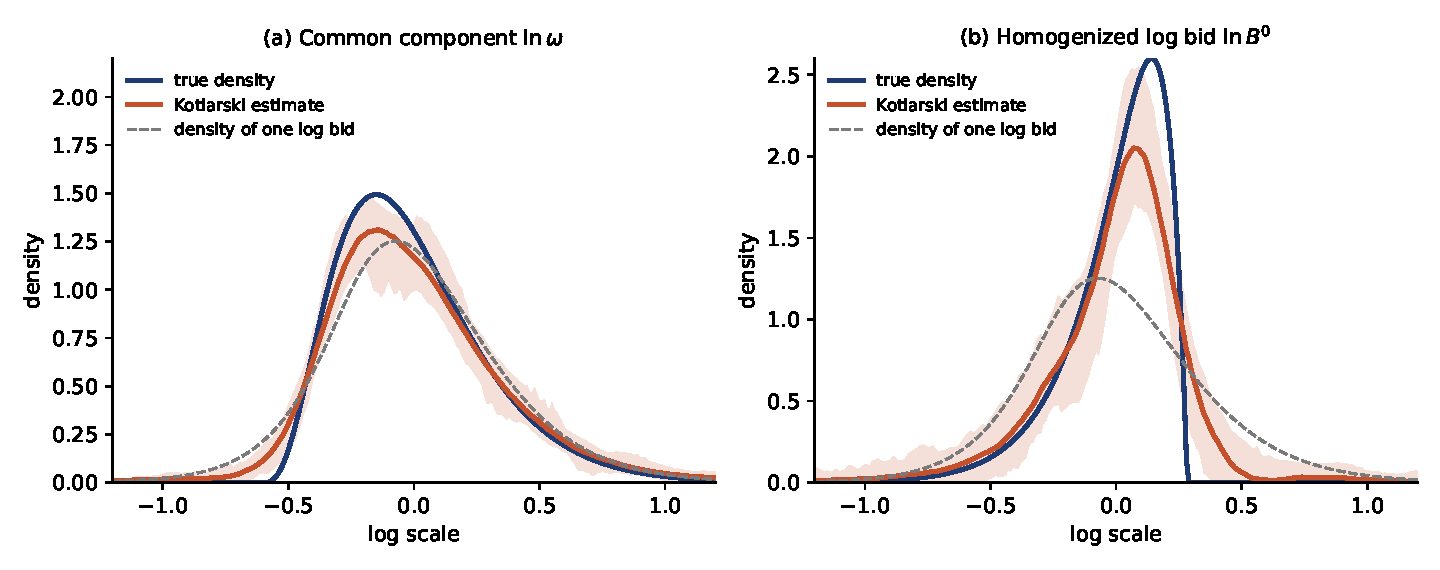
\includegraphics[width=\textwidth]{figures/ch15/kotlarski_demo.pdf}
\caption{Deconvolution of log bids with \eqref{eq:15-kotlarski} and the damped inverse
\eqref{eq:15-damped-inverse} (our simulation, seed 15703). $T=1{,}000$ auctions with four bidders of
one type. $\ln\omega$ is a standardized $\text{Gamma}(4)$ variable scaled to standard deviation $0.3$,
and $\ln B^0$ is a reflected standardized $\text{Gamma}(2)$ variable scaled to standard deviation
$0.2$. Characteristic functions average over all ordered pairs of bids. $T_c$ is chosen by
Krasnokutskaya's moment criterion on the grid $3,4,\dots,25$, and the largest value is usually chosen.
Lines show the median over 200 samples, bands the 5--95 percent range. The dashed curve is the density
of a single log bid.}
\label{fig:15-kotlarski}
\end{figure}

\subsubsection{Monte Carlo evidence}

The published Monte Carlo study is reported in figures only (Section 4.3, pp.~306--309). Costs are
multiplicative, $C=\omega A$, with distributions shaped like the estimated ones. Each sample has two
bidders of each type, as in the data, and $T=250$, $200$ or $150$ auctions, so each private component
is estimated from 500, 400 or 300 bids. The 5--95 percent bands of the estimated distributions
contain the true ones except in the smallest samples, where the bands are wide and miss small parts
of the true functions (p.~306).

The WP ran a more detailed study with tables, which we report next. Its design is additive,
$C=\omega+A$, with symmetric bidders (WP, Section 4.4). $A$ is
uniform with mean zero and variance $0.33$. $\omega$ follows a power distribution with exponent 3 and
mean $10.5$, with variances chosen so that bid functions have closed forms. Each sample has $T=400$
auctions with two bidders, and each experiment is replicated 500 times. Five cases are studied (WP,
Table 1b). Case 1 has independent costs. Case 2 has unobserved heterogeneity with $\Var(\omega)=0.04$
or $0.34$. Case 3 is APV, with bidders who observe only $C$. Cases 4 and 5 add correlation among
private components or between private and common components.
The estimator behaves as theory predicts (WP, Table 2b). With independent costs the estimated
$\Var(\omega)$ is $0.013$, with interval $[0.01,0.02]$, close to degenerate. The estimated markup is
$0.362$ against a true $0.38$. With heterogeneity, the estimated variances of $A$ are $0.321$ and $0.318$
against $0.33$. The estimated variances of $\omega$ are $0.0362$ and $0.335$ against $0.04$ and $0.34$.
Markups are $0.082$ and $0.092$ against $0.09$. WP Table 3b prints a true markup of $0.03$ for
$\Var(\omega)=0.34$, so the two tables of the paper disagree (see the notes to
\cref{tab:15-krasno-mc}). With APV data the procedure misreads the information
structure. The estimated markup is $0.18$ against a true $0.47$ in case 3a, and $0.33$ against $0.21$
in case 3b. With correlated components, the variance of $\omega$ is overstated and that of $A$
understated. The bias is negligible when the correlation is about 5 percent of $\Var(A)$ (WP, pp.
19--20).

The second experiment applies IPV and APV estimators to data with heterogeneity.
\Cref{tab:15-krasno-mc} reproduces the results. As $\Var(\omega)$ grows, both misspecified procedures
understate mean costs, overstate their variance, and overstate markups. Krasnokutskaya reports that the
bias becomes significant once the correlation of costs reaches about $0.3$ (WP, p.~21). Their bid
functions are flatter than the truth, and the IPV estimate is especially flat at the low end. A known
common component produces a bid distribution with thin tails, which IPV reads as extreme shading
at the bottom.

\begin{table}[htbp]
\centering
\caption{Misspecified estimators applied to data with unobserved heterogeneity (Krasnokutskaya 2004
working paper, Table 3b, not in the published article)}
\label{tab:15-krasno-mc}
\begin{tabular}{llccc}
\toprule
$\Var(\omega)$ & Procedure & $\E(C)$ & $\Var(C)$ & $\E(\text{markup})$\\
\midrule
0.04 & True model & 10.5 & 0.37 & 0.09\\
     & UH  & [10.44, 10.59] & [0.32, 0.41] & [0.078, 0.095]\\
     & APV & [10.37, 10.48] & [0.35, 0.44] & [0.097, 0.12]\\
     & IPV & [10.41, 10.5]  & [0.34, 0.44] & [0.95, 0.11]\\
\addlinespace
0.34 & True model & 10.5 & 0.67 & 0.03\\
     & UH  & [10.28, 10.64] & [0.63, 0.72] & [0.02, 0.038]\\
     & APV & [8.31, 9.57]   & [0.89, 1.02] & [0.042, 0.55]\\
     & IPV & [8.85, 9.84]   & [0.83, 0.96] & [0.4, 0.52]\\
\addlinespace
1    & True model & 10.5 & 1.33 & 0.01\\
     & UH  & [10.15, 10.76] & [1.27, 1.43] & [0.008, 0.014]\\
     & APV & [7.6, 8.8]     & [2.01, 2.27] & [0.033, 0.047]\\
     & IPV & [8.1, 9.2]     & [1.86, 2.05] & [0.31, 0.044]\\
\bottomrule
\end{tabular}

\smallskip
\begin{minipage}{0.93\textwidth}
\footnotesize \textit{Notes.} Additive design $C=\omega+A$, two symmetric bidders, 400 auctions, 500
replications. UH, APV and IPV denote estimators that assume unobserved heterogeneity, affiliated
private values and independent private values. Brackets give 5th and 95th pointwise percentiles of
the estimator. Entries are reproduced as printed. Four markup intervals look like decimal-point
typos in the source: $[0.95,0.11]$, $[0.042,0.55]$, $[0.4,0.52]$ and $[0.31,0.044]$. The true markup
at $\Var(\omega)=0.34$ is printed as $0.03$ here and as $0.09$ in WP Table 1b.
\end{minipage}
\end{table}

\subsubsection{Application: Michigan highway maintenance}

\casehead{Setting}
The Michigan Department of Transportation allocates road work by first-price sealed-bid auctions
(Section 5.1, pp.~306--307). It advertises a project 4 to 10 weeks before the letting, with a short
description of location, completion time and tasks. Firms can obtain a detailed description. The
department prepares an \emph{engineer's estimate} from the work required for each task, priced with
winning bids on similar past projects and deflated. Federal law requires the winning bid to be below
110 percent of this estimate, unless the state justifies an exception in writing. Bids and even
winning bids above the threshold appear in the data, so Krasnokutskaya treats the reserve as
nonbinding. Following the literature, she assumes bidders know how many rivals they face
(pp.~309--310).

\casehead{Data}
The sample covers maintenance projects with bituminous resurfacing as the main task, let between
February 1997 and December 2003, a total of 3,947 projects (p.~310). For each project she observes the
letting date, completion time, location, tasks, the identities and bids of all bidders, and the
engineer's estimate. Two arguments support the model. Resurfacing jobs are precisely specified and
simple, which favors private values. Their costs depend on elevation, curvature, traffic and the age
of the surface, which contractors see on site visits and the researcher does not. Firms differ mainly
in size, which every participant observes, so she allows two observable types. A bidder is
\emph{regular} if it won at least \$10 million of projects in each year of the data and has at least
100 employees (p.~310). She notes that this matches the industry's definition of a large bidder
(footnote 19). All other bidders are \emph{fringe}. The WP used a different definition, which the
published one replaces. There a regular bidder submits at least 12 bids per year, ranks in the top 10
percent of firms by employment and works in three or more specializations (WP, Section 5.2).

The number of bidders ranges from 1 to 11. More than 85 percent of projects have 2 to 6 bidders, and
the mean is 3.4 with standard deviation 1.3. About 75 percent of engineer's estimates lie between
\$100,000 and \$1,000,000, with 5 percent below and 20 percent above (p.~310).
\Cref{tab:15-krasno-desc} reproduces her descriptive table. The gap between the estimate and the
winning bid grows with the number of bidders. \emph{Money left on the table} is the gap between the two
lowest bids relative to the estimate. It averages 7 percent and falls from 11 to 4 percent as the
number of bidders rises (p.~311).

\begin{table}[htbp]
\centering
\caption{Michigan highway maintenance auctions: descriptive statistics by number of bidders
(Krasnokutskaya 2011, Table 1, and WP Table 1c)}
\label{tab:15-krasno-desc}
\begin{tabular}{lccccccc}
\toprule
Number of bidders & Overall & 1 & 2 & 3 & 4 & 5 & 6\\
\midrule
Number of observations & 3,947 & 71 & 673 & 1,126 & 1,026 & 365 & 192\\
\addlinespace
Engineer's estimate & 12.80 & 13.34 & 10.27 & 12.60 & 13.90 & 12.90 & 16.40\\
 & (2.35) & (2.88) & (1.41) & (3.02) & (2.26) & (1.79) & (3.39)\\
Winning bid & 11.10 & 14.12 & 10.00 & 11.80 & 12.90 & 11.80 & 15.20\\
 & (2.32) & (3.05) & (1.50) & (2.89) & (2.25) & (1.66) & (3.35)\\
Money left on the table & 0.07 & NA & 0.11 & 0.08 & 0.07 & 0.05 & 0.04\\
 & (0.05) & NA & (0.08) & (0.06) & (0.06) & (0.05) & (0.04)\\
Number of regular bidders & 1.92 & 0.79 & 1.43 & 1.65 & 2.07 & 2.16 & 2.29\\
 & (1.06) & (0.41) & (0.62) & (0.72) & (0.98) & (1.21) & (1.32)\\
\bottomrule
\end{tabular}

\smallskip
\begin{minipage}{0.93\textwidth}
\footnotesize \textit{Notes.} Means with standard deviations in parentheses. The engineer's estimate and the
winning bid are in hundreds of thousands of dollars. Money left on the table is the difference
between the lowest and second-lowest bids divided by the engineer's estimate. The overall column
includes projects with 7 to 11 bidders. The published Table 1 prints the columns for 2 to 6 bidders as
shown. Its overall column is misprinted, with 1.175 and 4.660 in every row, and its one-bidder column
prints the overall values. We take these two columns from WP Table 1c.
\end{minipage}
\end{table}

\casehead{Evidence of heterogeneity}
Krasnokutskaya first tests for heterogeneity (Section 5.2, p.~311). She conditions on a linear index
of observables estimated by ordinary least squares. The index contains the engineer's estimate,
duration, highway type, year, month and district dummies, and the number of tasks. The tests run
within cells defined by the main task and the number of bidders (Appendix A.3). The first test asks
whether two bids from the same auction are independent given the index, which is the null of IPV
against heterogeneity. The second asks whether two ratios built from four distinct bids are
independent, restriction (W3). This is the null of heterogeneity against APV. For resurfacing
projects with four regular bidders, the $p$-values are 0.03 and 0.52. IPV is rejected at the 5 percent
level, and heterogeneity is not rejected against APV. The test sample has 370 auctions with
estimates between \$350,000 and \$750,000 (footnote 21). \Cref{tab:15-krasno-index} reproduces the
index regressions.

\begin{table}[htbp]
\centering
\caption{Linear index of log bids on observables (Krasnokutskaya 2011, Table 2)}
\label{tab:15-krasno-index}
\begin{tabular}{lcc}
\toprule
 & Test subsample & Estimation subsample\\
\midrule
Constant & 0.375 & 0.327\\
 & (0.010) & (0.012)\\
Engineer's estimate & 0.8413 & 0.8113\\
 & (0.028) & (0.025)\\
Duration & 0.0011 & 0.0015\\
 & (0.0013) & (0.0011)\\
Tasks & 0.0014 & 0.0012\\
 & (0.0007) & (0.0009)\\
\addlinespace
$(n_{\text{regular}},n_{\text{fringe}})$ & (4,0) & (2,2)\\
Number of projects & 370 & 226\\
$R^2$ & 33\% & 17\%\\
\bottomrule
\end{tabular}

\smallskip
\begin{minipage}{0.8\textwidth}
\footnotesize \textit{Notes.} Ordinary least squares estimates of the mean of the log bid, with the figures in
parentheses as printed. Variables are labeled as in the source, which does not say whether the
engineer's estimate enters in logs. The test subsample is used for the specification tests and the
estimation subsample for the deconvolution.
\end{minipage}
\end{table}

The WP looked at the same correlation more directly. Its regressions of log bids in four-bidder
resurfacing projects are reproduced in \cref{tab:15-krasno-bids} (WP, Table 2c). Bids rise with the
engineer's estimate, distance to the site and the firm's backlog (``load remaining''), and fall with
the number of potential bidders. Fringe firms bid more. Adding auction dummies raises $R^2$ from
$0.857$ to $0.914$. The random-effects estimates attribute $\rho=0.48$ of the residual variance of log
bids to the auction level. The printed variance components imply a smaller share,
$\frac{0.16}{0.16+0.22}\approx0.42$. The text reports $R^2$ values of $0.81$ and $0.89$ for the same
regressions (WP, p.~25), which also differ from the table.
Common variation across bids in an auction that observables do not explain is the signature of
unobserved heterogeneity.

\begin{table}[htbp]
\centering
\caption{Regressions of log bids, four-bidder resurfacing projects (Krasnokutskaya 2004 working
paper, Table 2c, selected rows)}
\label{tab:15-krasno-bids}
\begin{tabular}{lccc}
\toprule
 & OLS & Auction dummies & Random effects\\
\midrule
Log (estimate) & 0.9100 & 0.9300 & 0.8800\\
 & (0.0530) & (0.1400) & (0.1300)\\
Duration & $-0.0210$ & $-0.0490$ & $-0.0210$\\
 & (0.0500) & (0.0250) & (0.0500)\\
Distance & 0.0312 & 0.0540 & 0.0270\\
 & (0.0160) & (0.0120) & (0.0160)\\
Log (load remaining) & 0.0310 & 0.0392 & 0.0270\\
 & (0.0157) & (0.0127) & (0.0144)\\
Number of potential bidders & $-0.1100$ & $-0.1330$ & $-0.1100$\\
 & (0.0310) & (0.0230) & (0.0290)\\
Fringe (dummy) & 0.2500 & 0.2800 & 0.2200\\
 & (0.1100) & (0.1200) & (0.1000)\\
Constant & 0.1750 & 0.1620 & 0.1680\\
 & (0.0580) & (0.0520) & (0.0480)\\
\addlinespace
$R^2$ & 0.857 & 0.914 & 0.917 (overall)\\
\bottomrule
\end{tabular}

\smallskip
\begin{minipage}{0.93\textwidth}
\footnotesize \textit{Notes.} Dependent variable $\ln B$. 947 bids. Standard errors in parentheses. Omitted rows
are length and dummies for marking, landscaping and signs. All columns include district and
regular-bidder dummies. Coefficients on auction-level variables in the auction-dummies column are
reproduced as printed. Random effects: $R^2$ within $0.00$, between $0.934$, $\sigma_u^2=0.16$,
$\sigma_\varepsilon^2=0.22$, $\rho=0.48$ as printed, although $\frac{\sigma_u^2}{\sigma_u^2+\sigma_\varepsilon^2}=0.42$.
These regressions are not in the published article.
\end{minipage}
\end{table}

Correlated bids could have other sources. Common values are unlikely, she argues, because simple
maintenance projects carry little project-level uncertainty. Collusion is harder to rule out, since
each test assumes a particular scheme (p.~311). Following \citet{PorterZona1993}, if only the winning
bid reflected a cost, the losing bids would be phony. She recovers the regular and fringe bid
distributions from the winning bid alone with the method of \citet{AtheyHaile2002}. These match the
distributions estimated from losing bids, which she reads as evidence against collusion (p.~312).

\casehead{Results}
Estimation uses the 226 projects with an engineer's estimate between \$300,000 and \$580,000, a
completion time of 3 to 6 months, and two regular and two fringe bidders (p.~312). Results for other
cells are described as qualitatively similar. Residual variation in observables is removed by
homogenization in logs, as in \cref{sec:15-uh-sep}. She regresses log bids on the observables of
\cref{tab:15-krasno-index} and deconvolves the residuals. Costs are then
$C_{it}=e^{z_t'\theta}\,\omega_tA_{it}$, and the fitted scaling factor $e^{z_t'\theta}$ is added back
for the variance decomposition and the comparisons (p.~312, footnote 22).

\Cref{tab:15-krasno-results} collects the main numbers (pp.~313--316). The heterogeneity component
$\omega$ has mean $0.98$ and standard deviation $0.204$. The \emph{common component}
$e^{z'\theta}\omega$, which combines the observed and the unobserved parts, has mean \$392,000 and
standard deviation \$78,890. The private components of the two types are similar. The fringe mean is
$1.06$, against the normalized regular mean of $1$, and the standard deviations are $0.14$ (regular)
and $0.13$ (fringe). Fringe firms thus have higher but slightly less dispersed costs. A test of equal
private-component distributions gives a $p$-value of 0.69 (p.~314). The text says that this rejects
equality at the 10 percent level, which a $p$-value of 0.69 does not support.

To split the variance of costs, she uses the exact identity for independent factors,
\[
\Var(\omega A)=\E[\omega^2]\E[A^2]-(\E\omega)^2(\E A)^2=(\E\omega)^2\Var(A)+(\E A)^2\Var(\omega)+\Var(\omega)\Var(A),
\]
and drops the last, second-order term (p.~314). She attributes $(\E\omega)^2\Var(A)$ to private
information and $(\E A)^2\Var(\omega)$ to common knowledge. Both terms are invariant to the
normalization, since $(\omega,A)\mapsto(c\,\omega,\frac{A}{c})$ leaves each unchanged (footnote 25).
For homogenized costs the private term accounts for almost 31 percent of the variance, and for 31.3
percent of the exact variance (footnote 26). For total costs, including the observed scaling factor,
it accounts for 34.4 percent (footnote 27). The rounded moments of regular bidders reproduce these
shares. For homogenized costs,
\[
\frac{(\E\omega)^2\Var(A)}{(\E\omega)^2\Var(A)+\Var(\omega)}
=\frac{0.98^2\times0.14^2}{0.98^2\times0.14^2+0.204^2}
=\frac{0.0188}{0.0188+0.0416}\approx0.31 .
\]
For total costs in thousands of dollars, the same ratio is
$\frac{392^2\times0.14^2}{392^2\times0.14^2+78.89^2}=\frac{3{,}012}{3{,}012+6{,}224}\approx0.33$, close
to the reported 34.4 percent. Private information therefore explains about a third of the variation
in costs, the 34 percent that \citet[p.~103]{HortacsuPerrigne2021} report for this article. The other
two thirds is information that all bidders share and the econometrician does not see.

The WP reported different figures from a different sample, and the published estimates supersede
them. Its sample had 487 larger and longer projects, with estimates between \$500,000 and \$900,000
and durations of 6 to 9 months (WP, p.~25). Its common component had mean \$654,000 and standard
deviation \$31,700, and its private components had standard deviations 0.22 and 0.23. Its text gave a
private share of ``almost 15\%'' (WP, p.~26), while its abstract and conclusion gave 25 percent.
Neither figure follows from its own moments. With $\E\omega=654$, $\sqrt{\Var(\omega)}=31.7$ and
$\sqrt{\Var(A)}=0.22$, the private term is $654^2\times0.22^2\approx20{,}700$ and the common term is
$31.7^2\approx1{,}005$, a private share near 95 percent.

Normalized markups $\frac{b-c}{c}$ range from 0.1 to 25 percent for regular bidders, with an average
of 8.4 percent. For fringe bidders they range from 0.1 to 18 percent, with an average of 6.1 percent
(p.~314). Fringe firms thus have higher costs, slightly less dispersed costs and lower markups than
regular firms, as \citet[p.~103]{HortacsuPerrigne2021} summarize. To measure inefficiency she draws
pseudo-samples of costs for 250 auctions with three bidders each, as printed. She computes bids from
the estimated bid functions and records how often the lowest bid does not come from the lowest cost.
Over 1,000 repetitions the probability of an inefficient outcome averages 5 percent, with a 95 percent
range of $[3.6,6.2]$. The misallocation raises the cost of procurement by 2 percent, with range
$[1.3,2.8]$ (p.~314). The WP's figure of 28 percent, with range $[26.6,30.3]$, came from pseudo-samples
of two regular and two fringe costs in its own sample (WP, pp.~25--28). It is superseded.

The IPV and APV estimators of \citet{GuerrePerrigneVuong2000} and \citet{LiPerrigneVuong2002},
applied to the same data, give larger markups and more dispersed costs (pp.~314--316). The average
markup of regular bidders is 14 percent under APV and 19 percent under IPV, against 8.4 percent under
heterogeneity. For fringe bidders the figures are 12.2, 16.5 and 6.1 percent. The variance of costs
estimated under heterogeneity is 18 percent lower than under APV and 22 percent lower than under IPV.
\Cref{fig:15-krasno-bidfn} shows why. Both misspecified bid functions lie above the heterogeneity
estimate, and their confidence bands meet its band only near the top of the support. The misspecified
estimators read common variation in bids as private information. They therefore infer lower costs and
larger markups from the same bids.

\begin{table}[htbp]
\centering
\caption{Michigan resurfacing auctions: estimates under unobserved heterogeneity (UH), APV and IPV
(Krasnokutskaya 2011, Section 5.3, with the superseded WP estimates)}
\label{tab:15-krasno-results}
{\small
\begin{tabularx}{\textwidth}{>{\raggedright\arraybackslash}Xcccc}
\toprule
 & \multicolumn{3}{c}{Published article} & WP (2004)\\
\cmidrule(lr){2-4}\cmidrule(lr){5-5}
 & UH & APV & IPV & UH\\
\midrule
Average markup $\frac{b-c}{c}$, regular bidders & 8.4\% & 14\% & 19\% & 7.5\%\\
Average markup $\frac{b-c}{c}$, fringe bidders & 6.1\% & 12.2\% & 16.5\% & 6\%\\
Probability of an inefficient allocation & 5\% [3.6, 6.2] & & & 28\% [26.6, 30.3]\\
Cost increase from misallocation & 2\% [1.3, 2.8] & & & \\
Cost variance under UH relative to column & & 18\% lower & 22\% lower & \\
\addlinespace
Common component, mean (s.d.) & \$392,000 (\$78,890) & & & \$654,000 (\$31,700)\\
Heterogeneity component $\omega$, mean (s.d.) & 0.98 (0.204) & & & \\
Private component $A$, s.d. regular, fringe & 0.14, 0.13 & & & 0.22, 0.23\\
Private component $A$, fringe mean (regular $=1$) & 1.06 & & & 1.2\\
Private share of variance, homogenized costs & 31\% & & & \\
Private share of variance, total costs & 34.4\% & & & 15\% or 25\%\\
\bottomrule
\end{tabularx}}

\smallskip
\begin{minipage}{0.93\textwidth}
\footnotesize \textit{Notes.} Published estimates use 226 projects with two regular and two fringe bidders,
engineer's estimates between \$300,000 and \$580,000 and durations of 3 to 6 months. Brackets give 95
percent ranges over 1,000 simulated pseudo-samples. The WP used 487 projects with estimates between
\$500,000 and \$900,000 and durations of 6 to 9 months. Its private share is 15 percent in the text and
25 percent in the abstract, and neither follows from its printed moments (see text). The WP also
reported inefficiency rates of 34 and 38 percent under IPV and APV and extra markups of \$61,000 and
\$33,000. Its cost variances under UH were 35 and 25 percent below IPV and APV (WP, pp.~25--28).
\end{minipage}
\end{table}

\begin{figure}[htbp]
\centering
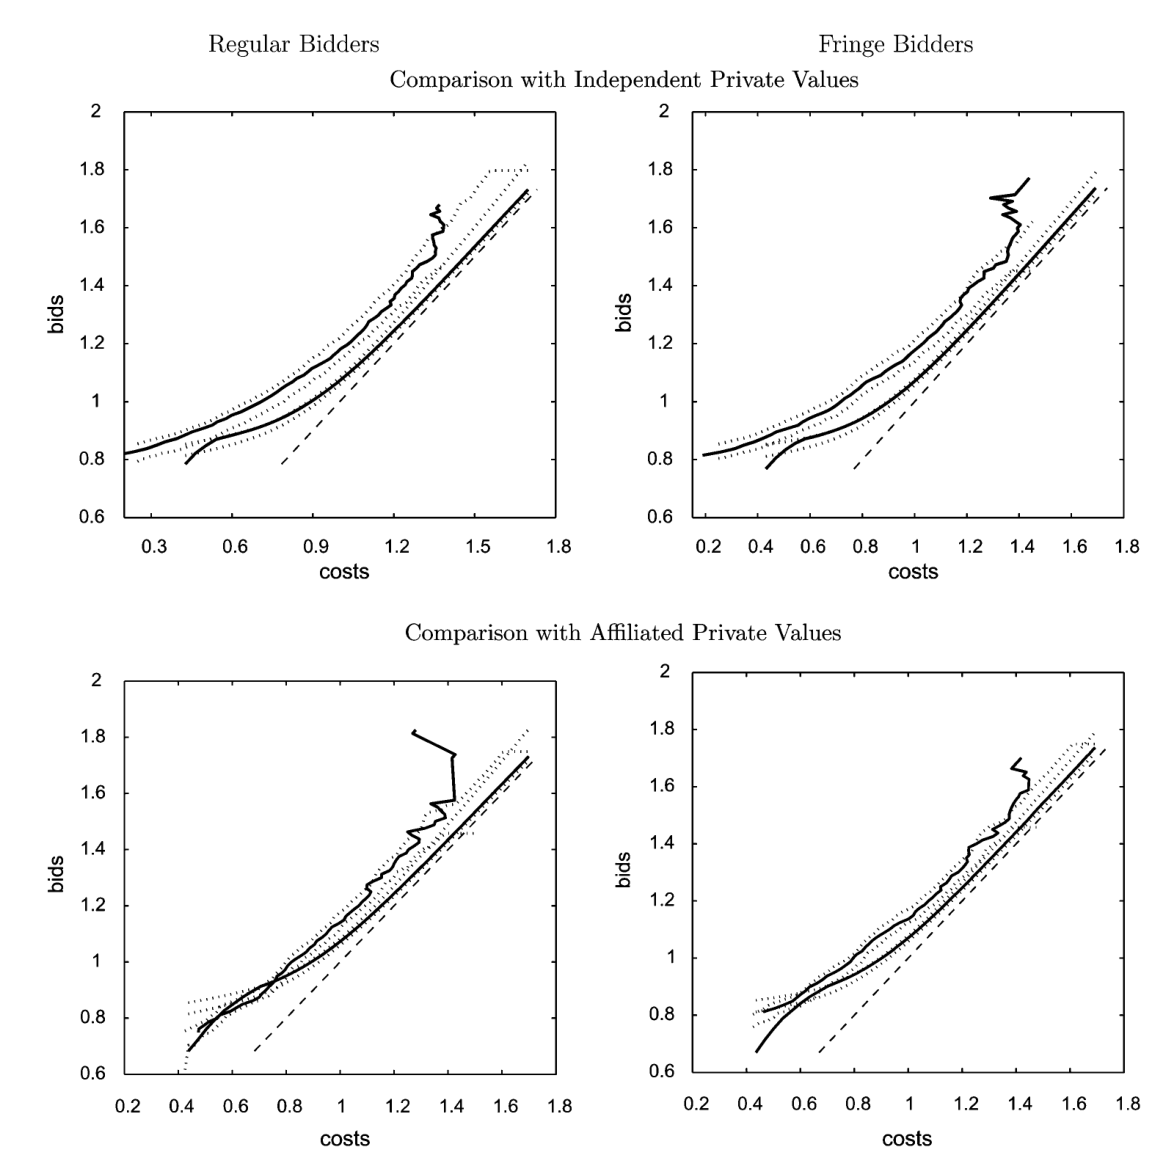
\includegraphics[width=0.86\textwidth]{figures/ch15/krasno_pub_fig5.png}
\caption{Expected bid functions, bids against costs in homogenized units, for regular (left) and
fringe (right) bidders. The top row compares the heterogeneity estimate with IPV, and the bottom row
compares it with APV. In each panel the dashed line is the diagonal. The lower solid line is the
estimate under unobserved heterogeneity, and the upper solid line is the misspecified estimate. Dotted
lines are pointwise 95 percent bootstrap bands. Source: Krasnokutskaya (2011), Figure 5.}
\label{fig:15-krasno-bidfn}
\end{figure}

\casehead{Reserve prices}
The estimates feed a design exercise (pp.~316--317). To avoid the complications of asymmetric
auctions, she uses the estimates for regular bidders only and treats bidders as symmetric. The
government minimizes the expected cost of procurement. If no bid falls below the maximum acceptable
price $r$, the project waits. Waiting costs $c_0$, which combines the cost of delay and the expected
cost of completing the work later. In the notation of \cref{sec:14-proc-other}, $c_0$ plays the role
of the buyer's value $u_0$. Suppose first that the government observes $\omega$. Costs then have the
distribution $F_C(c\mid\omega)=F_1\big(\frac{c}{\omega}\big)$ and density
$f_C(c\mid\omega)=\frac{1}{\omega}f_1\big(\frac{c}{\omega}\big)$. The virtual cost
\eqref{eq:14-virtual-cost} is
\[
J(c\mid\omega)=c+\frac{F_C(c\mid\omega)}{f_C(c\mid\omega)}
=c+\omega\,\frac{F_1(\frac{c}{\omega})}{f_1(\frac{c}{\omega})}
=\omega\,J_1\Big(\frac{c}{\omega}\Big),
\qquad J_1(a)=a+\frac{F_1(a)}{f_1(a)} .
\]
The optimal maximum price solves $J(r^*\mid\omega)=c_0$, so that
\[
r^*(\omega)=\omega\,J_1^{-1}\Big(\frac{c_0}{\omega}\Big).
\]
The reserve does not scale with $\omega$, because $c_0$ is fixed in dollars. This benchmark is case
(a) of her four candidates. In case (b) the government does not observe $\omega$. It chooses one reserve
that minimizes the expected cost averaged over $F_\omega$. Cases (c) and (d) use the cost distributions
estimated under IPV and APV. Each candidate is evaluated under the heterogeneity model. Since $c_0$ is
not observed, she reports results for several values.

\Cref{tab:15-krasno-reserve} reproduces her Table 4 for projects with an engineer's estimate of
\$400,000. Reserves based on IPV estimates raise the expected cost above the benchmark by 8.3 to 20.6
percent of $c_0$, which she rounds to 9 to 20 percent. Relative to the benchmark cost, the increase is 10
to 35 percent. The reserve of case (b) costs only
about 1 percent of $c_0$, or 1 to 2 percent of the benchmark. APV-based reserves do worse still. Both
misspecified models also imply too low a probability that any bid is submitted. For $c_0$ of at
least 150 percent of the mean cost, which she regards as the realistic range, accounting for
heterogeneity saves at least 16 percent of the benchmark cost (p.~317). This is large next to markups
of only 6 to 8 percent of costs.

\begin{table}[htbp]
\centering
\caption{Optimal reserve prices under alternative models (Krasnokutskaya 2011, Table 4)}
\label{tab:15-krasno-reserve}
{\small
\setlength{\tabcolsep}{4pt}
\begin{tabular}{clcccc}
\toprule
 & & \multicolumn{2}{c}{Unobserved heterogeneity} & & \\
\cmidrule(lr){3-4}
$c_0$ & & Benchmark (a) & Expected (b) & IPV (c) & APV (d)\\
\midrule
5 & Probability of a bid & 0.29 & 0.28 & 0.07 & 0.03\\
  & & (0.26, 0.31) & (0.25, 0.31) & (0.05, 0.09) & (0.02, 0.06)\\
  & Expected cost, \% of $c_0$ & 85.2 & 86.5 & 93.5 & 96.8\\
  & & (83, 87) & (85, 88) & (91, 95) & (95, 98)\\
  & Expected cost, \% of benchmark & & 101.4 & 109.7 & 113.6\\
\addlinespace
7 & Probability of a bid & 0.45 & 0.42 & 0.20 & 0.04\\
  & & (0.43, 0.46) & (0.40, 0.43) & (0.18, 0.21) & (0.03, 0.05)\\
  & Expected cost, \% of $c_0$ & 72.1 & 73.2 & 83.9 & 95.4\\
  & & (71.2, 73.5) & (72.3, 75.1) & (81.2, 84.7) & (94.3, 96.2)\\
  & Expected cost, \% of benchmark & & 101.6 & 116.4 & 132.4\\
\addlinespace
10 & Probability of a bid & 0.58 & 0.55 & 0.20 & 0.037\\
   & & (0.56, 0.59) & (0.54, 0.56) & (0.18, 0.21) & (0.03, 0.04)\\
   & Expected cost, \% of $c_0$ & 58.1 & 59.1 & 78.7 & 94.7\\
   & & (56.2, 59.5) & (57.8, 60.1) & (76.5, 79.7) & (94.0, 95.6)\\
   & Expected cost, \% of benchmark & & 101.6 & 135.5 & 163.0\\
\bottomrule
\end{tabular}}

\smallskip
\begin{minipage}{0.93\textwidth}
\footnotesize \textit{Notes.} Projects with an engineer's estimate of \$400,000, regular bidders treated as
symmetric. $c_0$ is the cost of not awarding the project today, in hundreds of thousands of dollars.
(a) The government observes $\omega$. (b) One reserve minimizes the cost averaged over $F_\omega$. (c),
(d) Reserves computed from IPV and APV estimates. All candidates are evaluated under the heterogeneity
estimates. Intervals in parentheses as printed.
\end{minipage}
\end{table}

\casehead{Tests of the assumptions and robustness}
Her Table 3 reports tests of the restrictions of Proposition 2 (pp.~317--318). The ratio test (W3)
of Section 5.2 gives a $p$-value of 0.52. Independence of the private components from $\omega$ gives
0.81 (bootstrap) and 0.75 (subsampling). Independence of the private components across bidders gives
0.43 and 0.63. The text adds a $p$-value of 0.63 for the test of part 1 of Proposition 2. None of the
tests rejects.
One robustness check addresses dynamics. Capacity constraints would link bids across auctions and bias
the estimated joint characteristic function. She re-estimates the model on projects for which every
regular bidder's backlog lies between 30 and 75 percent of the largest backlog observed in the data.
The sample shrinks and the estimates are less precise, but the variance decomposition and the biases
from misspecification are similar (pp.~318--319). The WP adds a fit check. Pseudo-bids simulated from
the estimated model reproduce the estimated densities of actual bids, with the largest gap near the
mode (WP, p.~28, Figure 3c).

\subsubsection{Assessment}

Krasnokutskaya's paper gave the first nonparametric identification result for first-price auctions
with unobserved heterogeneity. It turned the repeated-measurement idea into an auction estimator, and it
quantified how IPV and APV estimators err. In Michigan resurfacing, private information explains only
about a third of cost variation, 34 percent of the variation in total costs (p.~319). The remaining
two thirds is common knowledge among bidders. Ignoring it raises the estimated average markup of
regular bidders from 8.4 percent to 14 percent (APV) or 19 percent (IPV). Reserve prices based on the
misspecified models would raise procurement costs by 10 to 63 percent of the benchmark. The asymmetry
between regular and fringe firms matters less, with inefficient awards in 5 percent of auctions at a
cost of 2 percent. \citet[p.~103]{HortacsuPerrigne2021} summarize the published findings in the same
terms. The WP's figures differ, with a 28 percent inefficiency rate and a private share of 15 or 25
percent, and the published article replaces them.

The approach has four limits. First, heterogeneity must be scalar and enter by a known separable
form, and the two-dimensional extension needs four bids. Second, independence of $\omega$ and $\bm A$
and across bidders is essential. Her tests do not reject it (Table 3), but they have limited power,
and the model leaves no room for affiliation among the private components. Third, estimation is cell
by cell in $(n,n_1)$ and covariates, with slow rates, and the published estimates rest on 226 projects.
\citet[footnote 22]{AtheyLevinSeira2011} give this reason for not using the method on timber data.
``[O]ne would want to estimate the model separately for each vector of participants $(n_L,n_M)$ and we
simply don't have the data to do this.'' Fourth, the number of bidders is taken as exogenous. Entry
that responds to $\omega_t$ would violate (D1), and Krasnokutskaya leaves participation to separate
work.

\citet{KrasnokutskayaSeim2011} add participation in later work on California highway procurement,
where small firms receive a bid preference \citep[p.~123]{HortacsuPerrigne2021}. They estimate an
entry model of the \citet{LevinSmith1994} type with cost asymmetries. Entry costs are 2.2 to 3.9
percent of the engineer's estimate for small firms and 3.1 to 3.3 percent for large firms. The state
aims to award 25 percent of procurement dollars to small firms. The authors first evaluate this goal for
one illustrative project \citep[pp.~2655--2656, Figure~1]{KrasnokutskayaSeim2011}. With fixed
participation, reaching the goal on that project requires a small-firm discount of more than 50 percent,
at a predicted cost increase of 0.23 percent. Allowing entry to respond, that discount would deter large
firms and raise the cost by 7.8 percent. A discount of about 20 percent then reaches the goal on the same
project, and the procurement cost rises by 3.2 percent. These figures describe a single project. For all
projects together, the article's text reports that a 15 percent discount approximately meets the aggregate goal, at a
cost increase of 1.4 percent (p.~2678). Their Table~11 instead lists, for the same 15 percent discount, a
small-firm share of work of 31.9 percent and a cost increase of 2.1 percent (p.~2679). The article does
not reconcile the two sets of numbers. \Cref{sec:14-proc-other} discusses the theory of such preferences. Later work relaxes separability.
\citet{HuMcAdamsShum2013} identify nonseparable heterogeneity from three bids per auction (as described
by \citealp{Roberts2013}, p.~5). \citet{Asker2010} applies the deconvolution to knockout bids in a
stamp cartel (\cref{sec:13-asker-structural}).

\subsection{Parametric approaches}\label{sec:15-uh-param}

A parametric first step trades flexibility in the distributions for flexibility in how covariates
and heterogeneity enter. \citet{AtheyLevinSeira2011} specify Weibull bid distributions conditional on a
Gamma-distributed multiplicative component, which integrates out in closed form
(\cref{sec:15-als}, \cref{prop:15-als-lik}). Values then follow from the first-order condition at any
$\omega$, as in \cref{thm:15-krasno}. The parametric form lets heterogeneity affect types
differently and keeps estimation feasible with many participant configurations
\citep[Section 6.1.2]{AtheyHaile2007}. \citet{RobertsSweeting2013} estimate values with heterogeneity
in values and entry costs by simulated maximum likelihood with importance sampling (as described by
\citealp{Roberts2013}, p.~6). \citet{HongShum2002} model the median of the bid distribution as a normal
random variable whose mean depends on the number of bidders (as described by
\citealp{Krasnokutskaya2011}, p.~296). Finite mixtures of parametric distributions offer a middle
ground \citep[eqs. (6.7)--(6.9)]{AtheyHaile2007}. In all of these, identification of the
heterogeneity distribution leans on functional form.

\subsection{Reserve prices as a control for quality: Roberts (2013)}\label{sec:15-roberts}

\casehead{Idea}
Every method so far uses only bidders' behavior. \citet{Roberts2013} uses the seller's behavior. A
seller who knows the object well probably observes what the bidders observe. If the reserve price
rises with the unobserved quality, then reserve prices reveal it. The logic is that of a control
function, close to the use of investment as a proxy for productivity by \citet{OlleyPakes1996}.
\citet{Roberts2013} credits the suggestion to Athey and Haile, and \citet[footnote 56]{AtheyHaile2007}
point to restrictions from the seller's side as a direction worth exploring. His motivating evidence
is old. In the eggplant data of \citet{LaffontOssardVuong1995}, winning bids and reserve prices move
in tandem across auctions (\citealp{Roberts2013}, p.~7, citing their Appendix figure, reproduced in
\cref{fig:15-lov-reserve}).

\casehead{Model}
In auction $t$ there are $N_t$ bidders with symmetric independent private values. Observed
characteristics $Z_t$ and the scalar $\omega_t$ are known to the seller and the bidders, and the
econometrician observes only $Z_t$. Values are drawn from $F_V(\cdot\mid Z_t,\omega_t)$, which may depend
on $\omega_t$ in any way, but not on $N_t$. The seller sets the reserve price $r_t=m(Z_t,\omega_t)$ with
the same function $m$ in every auction. The bidders counted in $N_t$ include those with values below
$r_t$.

\begin{assumption}[\citealp{Roberts2013}, Assumption S1]\label{ass:15-roberts}
For every $z$, $m(z,\omega)$ is strictly increasing in $\omega$.
\end{assumption}

Reserves need not be optimal. Monotonicity is nevertheless what optimal reserves deliver when higher
$\omega$ makes higher values strictly more likely. Recall the virtual valuation \eqref{eq:14-psi} and write it conditionally on $\omega$ as
$\psi(t\mid\omega)=t-\frac{1-F_V(t\mid\omega)}{f_V(t\mid\omega)}$. The optimal reserve solves
$\psi(r^*\mid\omega)=v_0$, where $v_0$ is the seller's value (\cref{cor:14-optimal-reserve}).

\begin{proposition}[\citealp{Roberts2013}, Proposition 1]\label{prop:15-roberts1}
Suppose $\psi(t\mid\omega)$ is strictly increasing in $t$ for every $\omega$. If $V$ and $\omega$ are
affiliated, the optimal reserve price is nondecreasing in $\omega$. If they are strictly affiliated, so that the
likelihood ratio inequality below is strict for all $v_1<v_2$ and $\omega_1<\omega_2$, the optimal reserve price
is strictly increasing in $\omega$.
\end{proposition}

\begin{proof}
Take $\omega_1<\omega_2$. By \cref{prop:14-affil-mlrp}, affiliation gives the monotone likelihood ratio
property. For $v_1<v_2$,
$\frac{f_V(v_2\mid\omega_1)}{f_V(v_1\mid\omega_1)}\le\frac{f_V(v_2\mid\omega_2)}{f_V(v_1\mid\omega_2)}$,
strictly under strict affiliation. Integrating over $v_2>v_1$ gives
$\frac{1-F_V(v_1\mid\omega_1)}{f_V(v_1\mid\omega_1)}\le\frac{1-F_V(v_1\mid\omega_2)}{f_V(v_1\mid\omega_2)}$,
so the inverse hazard is nondecreasing in $\omega$ and $\psi(t\mid\omega_2)\le\psi(t\mid\omega_1)$ for every $t$.
Integration preserves strict inequality, so both inequalities are strict under strict affiliation. Let $r_1$
solve $\psi(r_1\mid\omega_1)=v_0$. Then $\psi(r_1\mid\omega_2)\le v_0$. Since $\psi(\cdot\mid\omega_2)$ is
strictly increasing, the solution $r_2$ of $\psi(r_2\mid\omega_2)=v_0$ satisfies $r_2\ge r_1$. Under strict
affiliation $\psi(r_1\mid\omega_2)<v_0$, and therefore $r_2>r_1$.
\end{proof}

Affiliation alone does not deliver \cref{ass:15-roberts}. Independent $V$ and $\omega$ are affiliated, yet the
optimal reserve then does not move with $\omega$. With $V$ uniform on $[0,1]$ and $v_0=0$, for example,
$r^*=\frac12$ for every $\omega$. The proof in \citet[Appendix~B]{Roberts2013} writes the affiliation inequality
as strict, which is the strict case of the proposition.

The second result is the identification theorem. Partition $Z=(Z_0,Z_1)$.

\begin{proposition}[\citealp{Roberts2013}, Proposition 2]\label{prop:15-roberts2}
Let \cref{ass:15-roberts} hold. Suppose (i) there is a value $z_1^*$ such that $m(z_0,z_1^*,\omega)=\omega$
for all $z_0$ and $\omega$, and (ii) $\omega$ is independent of $Z_1$ conditional on $Z_0$. Then reserve prices
identify $F_{\omega\mid Z_0}$, the function $m$ and each realization $\omega_t$. Suppose in addition that the
number $N$ of potential bidders is known and that unsold auctions are recorded. Then transaction prices identify
$F_V(v\mid Z,\omega)$ for every $v\ge m(Z,\omega)$, including the mass $F_V\big(m(Z,\omega)\mid Z,\omega\big)$, in
first-price and second-price (or ascending) auctions.
\end{proposition}

\begin{proof}
\emph{Step 1 (the law of $\omega$).} By (i) and (ii),
\[
\Pr(r_t\le u\mid Z_0=z_0,Z_1=z_1^*)=\Pr(\omega_t\le u\mid Z_0=z_0,Z_1=z_1^*)=F_{\omega\mid Z_0}(u\mid z_0).
\]
\emph{Step 2 (the function $m$).} For any $z_1$, monotonicity and (ii) give
\[
F_{\omega\mid Z_0}(u\mid z_0)=\Pr\big(m(z_0,z_1,\omega_t)\le m(z_0,z_1,u)\mid z_0,z_1\big)=F_{r\mid Z}\big(m(z_0,z_1,u)\mid z_0,z_1\big),
\]
so $m(z_0,z_1,u)=F_{r\mid Z}^{-1}\big(F_{r\mid Z}(u\mid z_0,z_1^*)\mid z_0,z_1\big)$ is identified.
\emph{Step 3 (realizations).} Since $m$ is strictly increasing in $\omega$, each observed $(r_t,Z_t)$
reveals $\omega_t=m^{-1}(Z_t,r_t)$.
\emph{Step 4 (values).} Treat $(Z_t,\omega_t)$ as observed covariates. For fixed $(Z,\omega)$ the
reserve $m=m(Z,\omega)$ is fixed, so transaction prices are censored at it. For $v\ge m$ let $W(v)$ be the
probability that the object goes unsold or sells at a price of at most $v$. Unsold auctions enter $W$, which
is why they must be recorded. In a second-price or ascending auction, the second-highest of the $N$ values is
at most $v$ exactly when this event occurs, so $W(v)=\Lambda_{N-1:N}\big(F_V(v\mid Z,\omega)\big)$. Inverting
$\Lambda_{N-1:N}$, which requires $N$, gives $F_V(v\mid Z,\omega)$. In a first-price auction whose bidders know $N$
but not who participates, as in \cref{sec:15-gpv-reserve}, let $\xi$ be the inverse bid function above the
reserve. The event occurs at a bid level $b\ge m$ when every potential bidder
stays out or bids at most $b$, so $W(b)=F_V\big(\xi(b)\mid Z,\omega\big)^N$. A bidder's win probability is
$W(b)^{\frac{N-1}{N}}$, and the first-order condition gives $\xi(b)=b+\frac{N}{N-1}\frac{W(b)}{W'(b)}$, as in
\eqref{eq:15-winbid-xi}. Then $F_V\big(\xi(b)\mid Z,\omega\big)=W(b)^{\frac1N}$. In both formats $W(m)$, the
probability of no sale or a sale at the reserve, gives the mass at $m$.
\end{proof}

With less data the conclusion narrows. Without $N$ the transformation from $W$ to $F_V$ is unknown, and without
the unsold auctions the prices of sold objects do not determine $W$. In second-price and ascending auctions that
record the number of actual bidders, transaction prices still identify the value distribution truncated at the
reserve, by \cref{prop:15-reserve-ident}(i).

\Citet[Proposition 2]{Roberts2013} states the result without the restriction $v\ge m(Z,\omega)$ and
without the requirements on $N$ and on unsold auctions. His proof cites \citet[Theorems 1 and 6]{AtheyHaile2002},
which assume no binding reserve. Below the
reserve, no bid is recorded and the data carry no information about $F_V(\cdot\mid Z,\omega)$, as in
\cref{thm:15-gpv-reserve}. The reserve does bind in his data, since 107 of 1,117 cars in one subsample
go unsold.

The normalization (i) holds in many functional forms, for example $r=z\,\omega$ or $r=z+\omega$ at a
suitable $z$ (\citealp{Roberts2013}, footnote 6). Unlike \cref{thm:15-krasno}, the result allows values
to depend on $\omega$ in any way. Among bids it needs only the transaction price, together with $N$ and the
record of unsold auctions. It requires instead that the
reserve depend on nothing that the bids do not reflect.

\casehead{Setting and data}
The data come from a wholesale used-car auction house in Suwon, South Korea, which held weekly auctions
between October 10, 2001 and November 27, 2002 (\citealp{Roberts2013}, Section 3).
Only registered dealers may bid, and more than 380 were registered. The house charges the seller \$50
per car and collects 2.2 percent of the price from each side if the car sells. Sellers set reserve
prices, usually with guidance from the house. Dealers receive car descriptions three days ahead and
inspect the cars for three hours or more before the auction. The format is a button auction with
reentry. The price rises by \$30 every three seconds while at least two buttons are pressed, and bidders
cannot see when rivals drop out. Of 28,334 passenger cars, Roberts studies 4,943 automatic
five-passenger sedans. Hyundai, Daewoo and Kia account for 42, 39 and 18 percent of auctions. The
average winning bid is \$3,661.83, the average reserve \$3,361.26, and 5.37 bidders bid on the
average car (\citealp{Roberts2013}, Table 1). Among bids, only the transaction price is recorded,
together with the identities of the winner and the runner-up and the number of bidders.

\casehead{Evidence for the assumptions}
Several facts support the model (\citealp{Roberts2013}, pp.~13--19). In regressions of the log
winning bid on car characteristics and dummies, $R^2$ rises from $0.903$ to $0.979$ when the log
reserve is added. The log reserve alone gives $0.966$ (Table 2). The residuals of winning bids and of
reserves, after both are regressed on characteristics, have correlation $0.890$, against a raw
correlation of $0.983$. For 107 unsold cars among 1,117 auctioned between October 10 and December 27,
2001, the same residual correlations are $0.942$ for the highest bid and $0.943$ for the average bid.
The reserve does not predict failure to sell. Its coefficient in a logit is $0.232$ with standard error
$0.263$ (Table 4). Moving the reserve from its 25th to its 75th percentile raises the failure
probability by about 2 percentage points. Reserves do not rise with the number of bidders, which a
signaling model of reserves would predict \citep{CaiRileyYe2007}. About four of the roughly five
bidders per car bid above the reserve, so the co-movement is not mechanical. Bidders look symmetric.
Three quarters of them buy 17 or fewer cars over 59 auction days.

\casehead{Estimation}
For Hyundai Sonatas, Roberts specifies $m(Z_1,\omega)=\mu(X;\vartheta)+\omega$ with $\E[\omega X]=0$
(p.~19). Here $X$ collects age and mileage. The function $\mu$ is quadratic in them, including their
interaction. The residual of this regression estimates $\omega_t$. The distribution of transaction prices $P_t$ given
$Z=(Z_1,\hat\omega)$ is estimated by a kernel estimator of a conditional distribution (his eq. (3)),
\[
\hat F_{P\mid Z=z}(v)=\frac{\sum_{t=1}^T\tilde{\mathcal K}_1\big(\frac{v-P_t}{h}\big)\,\mathcal K_2\big(\frac{z-Z_t}{h}\big)}{\sum_{t=1}^T\mathcal K_2\big(\frac{z-Z_t}{h}\big)},
\]
where $\tilde{\mathcal K}_1$ is the integral of a kernel $\mathcal K_1$. Gaussian kernels and Silverman's
bandwidth are used. Bid increments are ignored, so the transaction price is the second-highest of $N$
values, and $\hat F_V(v\mid z)=\Lambda_{N-1:N}^{-1}\big(\hat F_{P\mid Z=z}(v)\big)$ (his eq. (2), our
\eqref{eq:15-Lambda}). By \cref{prop:15-roberts2}, this inversion is valid for $v$ at or above the
reserve, and only if unsold auctions enter $\hat F_{P\mid Z}$ as described in Step 4. Roberts does not
treat the reserve as a censoring point. Since about four of the roughly five bidders per car bid above
the reserve, the censoring mainly affects the lower tail of the estimated value distribution.
Consistency with a generated regressor follows from conditions in \citet{Matzkin2003}. Roberts pools months with similar numbers of unique bidders, whose average is
$62.6$. He drops auctions with more than eight bidders, which keeps over 92 percent of them, and sets
$N=8$. The restricted sample has 454 Sonatas, with mean winning bid \$3,574.38, mean reserve
\$3,320.22, mean age $84.10$ months and $4.83$ unique bids per car (Table 5). In this sample the
adjusted $R^2$ of the log winning bid rises from $0.773$ to $0.971$ with the reserve, and the residual
correlation is $0.9343$ against a raw $0.9835$.

\casehead{Results}
\Cref{fig:15-roberts-cdf} shows estimated value distributions for a seven-year-old Sonata with 100,000
km. Ignoring heterogeneity produces a much more dispersed distribution. Controlling for it, the
distributions at the 10th, 50th and 90th percentiles of $\omega$ are ordered by first-order stochastic
dominance. Their means are \$1,919.61, \$2,426.20 and \$2,971.17, with bootstrap 95 percent intervals
$[1{,}904.37,1{,}937.11]$, $[2{,}406.88,2{,}448.65]$ and $[2{,}946.99,2{,}999.08]$ (p.~22). With $N=7$ the
means are \$2,168.82, \$2,542.19 and \$3,146.35, and with $N=9$ they are \$1,871.81, \$2,326.22 and
\$2,788.02 (footnote 9). A parametric alternative with lognormal values and a Poisson number of bidders
gives \$1,758.45, \$2,184.41 and \$2,864.57, with an estimated mean of $8.84$ bidders (footnote 10).

\begin{figure}[htbp]
\centering
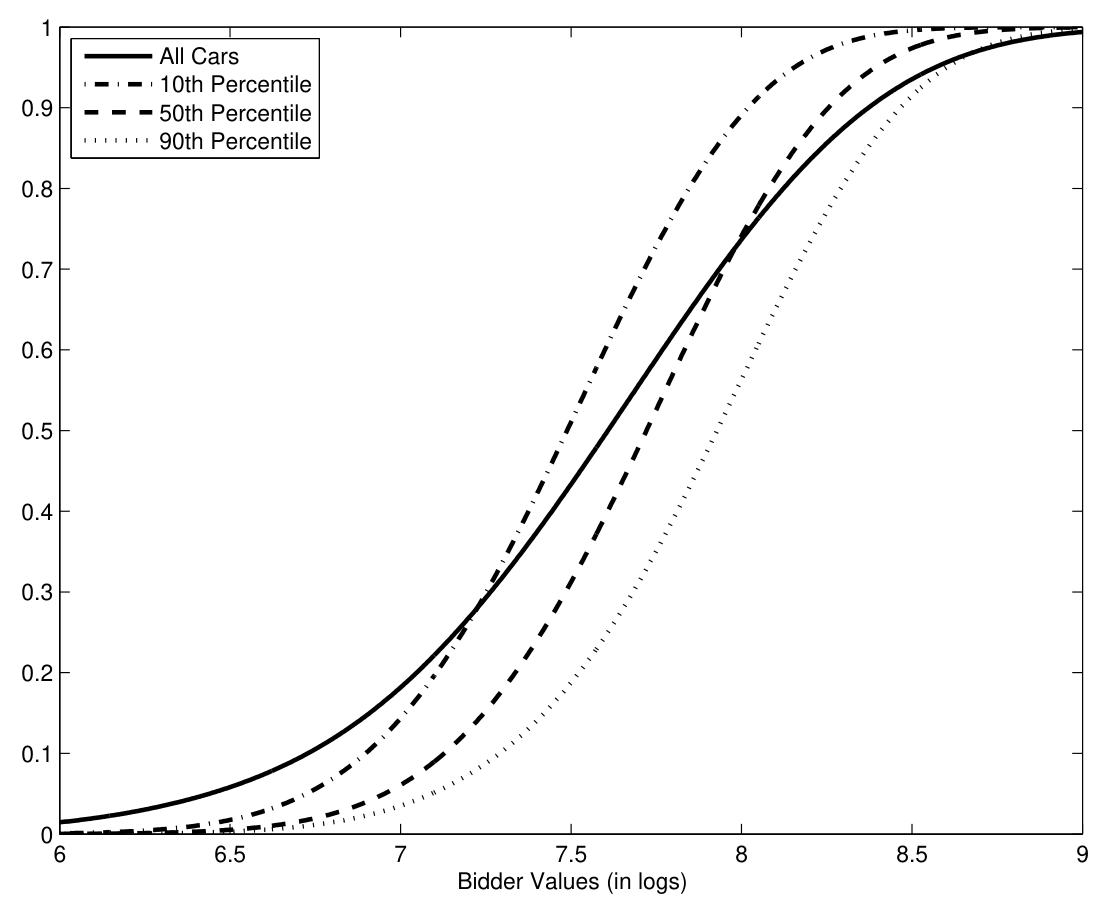
\includegraphics[width=0.62\textwidth]{figures/ch15/roberts_fig1.png}
\caption{Estimated value distributions (log values) for seven-year-old automatic Hyundai Sonatas with
100,000 km. Solid line: ignoring unobserved heterogeneity. Other lines: controlling for it at the 10th,
50th and 90th percentiles of $\omega$. Source: Roberts (2013), Figure 1 (June 2013 working-paper version).}
\label{fig:15-roberts-cdf}
\end{figure}

\casehead{Counterfactuals}
Roberts asks how much of the attainable value sellers capture and through which channels. He sets the
seller's value to $v_0=\gamma r$ for $\gamma\in\{0,0.25,0.5,0.75\}$ and simulates revenues with
$N=8$. \Cref{tab:15-roberts-reserve} reproduces his Table 6. Ignoring heterogeneity overstates the
dispersion of values and pushes the estimated optimal reserve up. A sufficient condition is hazard rate
dominance. Let $\lambda_C$ and $\lambda_{NC}$ be the hazard rates of the value distributions estimated
with and without the control, and suppose $\lambda_C(r)>\lambda_{NC}(r)$ for all $r$. The optimal
reserve with the control solves $r_C=v_0+\frac{1}{\lambda_C(r_C)}<v_0+\frac{1}{\lambda_{NC}(r_C)}$, so
$\psi_{NC}(r_C)<v_0$. Regularity then gives $r_{NC}>r_C$ (\citealp{Roberts2013}, footnote 13). With
actual reserves, the mean seller captures between 88.42 and 92.23 percent of the value of the optimal
auction with the same bidders, depending on $\gamma$. Using the ``optimal'' reserves computed while
ignoring heterogeneity would lower the mean share to between 85.53 and 88.93 percent. The text
summarizes the first result as ``around 94\%'' (p.~25), above every mean and median in the table. The
figure is close to the 90th-percentile column, 93.08 to 94.51 percent. The text also says that 90
percent of sellers achieve more than 83 percent, which matches the 10th percentile of 83.69 at
$\gamma=0$.

\begin{table}[htbp]
\centering
\caption{Optimal reserve prices and the share of value captured by sellers (Roberts 2013, Table 6)}
\label{tab:15-roberts-reserve}
{\small
\setlength{\tabcolsep}{4pt}
\begin{tabular}{ccccccccccc}
\toprule
 & \multicolumn{2}{c}{Difference in optimal reserve} & \multicolumn{4}{c}{Actual reserves (\%)} & \multicolumn{4}{c}{Reserves ignoring UH (\%)}\\
\cmidrule(lr){2-3}\cmidrule(lr){4-7}\cmidrule(lr){8-11}
$\gamma$ & Overall & Median & Mean & 10th & 50th & 90th & Mean & 10th & 50th & 90th\\
\midrule
0.00 & \$221.57 & \$77.21 & 88.42 & 83.69 & 89.18 & 93.08 & 85.53 & 77.37 & 94.08 & 94.70\\
     & (25.36) & (24.89) & (0.19) & (0.33) & (0.18) & (0.14) & (0.13) & (0.17) & (0.03) & (0.04)\\
0.25 & 258.52 & 90.20 & 90.66 & 86.69 & 91.69 & 93.53 & 86.58 & 74.62 & 94.10 & 94.70\\
     & (23.16) & (25.52) & (0.18) & (0.38) & (0.13) & (0.05) & (0.11) & (0.13) & (0.03) & (0.03)\\
0.50 & 239.72 & 98.45 & 92.23 & 86.98 & 93.69 & 94.25 & 87.60 & 74.05 & 94.05 & 94.70\\
     & (21.35) & (21.01) & (0.20) & (0.64) & (0.04) & (0.03) & (0.08) & (0.11) & (0.03) & (0.02)\\
0.75 & 236.03 & 123.57 & 91.81 & 85.84 & 93.45 & 94.51 & 88.93 & 80.42 & 94.04 & 94.71\\
     & (21.79) & (22.12) & (0.20) & (0.76) & (0.07) & (0.04) & (0.07) & (0.08) & (0.03) & (0.02)\\
\bottomrule
\end{tabular}}

\smallskip
\begin{minipage}{0.93\textwidth}
\footnotesize \textit{Notes.} $v_0=\gamma r$, with $r$ the observed reserve. ``Overall'' is the average
difference across all cars, and ``Median'' the average for cars with $\omega$ within half a standard
deviation of its median. The paper's column header, and its definition on p.~24, write the difference
as $R^*_C-R^*_{NC}$. The table note describes it as the optimal reserve ignoring heterogeneity minus
the optimal reserve controlling for it. The text and its footnote 13 say that ignoring heterogeneity
raises the optimal reserve. The positive entries agree with the note, which we follow. The remaining columns give the percentage of the value of the
optimal auction captured with actual reserves and with the ``optimal'' reserves that ignore
heterogeneity. Bootstrap standard errors (100 repetitions) in parentheses, in percentage points for
percentages.
\end{minipage}
\end{table}

\Cref{tab:15-roberts-channels} reproduces Table 7, which decomposes the value of the platform with
$\gamma=0$. Let $\pi^N_{r}$ denote revenue with $N$ bidders and reserve $r$. The first row is the gain
$\pi^{N+1}_{r=r^*}-\pi^N_{r=0}$ from one more bidder together with an optimal reserve. The next rows split
the gain into the extra bidder, $\pi^{N+1}_{r=0}-\pi^N_{r=0}$, and the reserve,
$\pi^{N+1}_{r=r^*}-\pi^{N+1}_{r=0}$. The extra bidder dominates, as the theorem of
\citet{BulowKlemperer1996} suggests (\cref{prop:14-bk}). With four bidders, the extra bidder is
worth $\frac{94.49}{5.51}\approx17.1$ times as much as the optimal reserve when heterogeneity is
controlled for, and $\frac{81.89}{18.11}\approx4.5$ times as much when it is not. With five bidders the ratios are $26.1$ and $5.1$.
The text reports 17.5 and 4.6 ``when there are five bidders'' (p.~26), close to our ratios for $N=4$, where
the extra bidder makes five.
Ignoring heterogeneity overstates the role of reserves and understates the role of competition.

\begin{table}[htbp]
\centering
\caption{Channels through which sellers gain from the auction house (Roberts 2013, Table 7)}
\label{tab:15-roberts-channels}
\begin{tabular}{lcccccc}
\toprule
$N$ & 2 & 3 & 4 & 5 & 6 & 7\\
\midrule
\multicolumn{7}{l}{\emph{Controlling for unobserved heterogeneity}}\\
Gain $\pi^{N+1}_{r=r^*}-\pi^{N}_{r=0}$ (\$) & 725.94 & 435.5 & 307.89 & 233.09 & 189.07 & 160.59\\
 & (14.95) & (8.98) & (6.56) & (5.13) & (4.23) & (3.49)\\
Share from extra bidder (\%) & 87.71 & 91.91 & 94.49 & 96.31 & 97.31 & 97.97\\
 & (0.41) & (0.39) & (0.34) & (0.31) & (0.31) & (0.34)\\
Share from optimal reserve (\%) & 12.29 & 8.09 & 5.51 & 3.69 & 2.69 & 2.03\\
 & (0.41) & (0.39) & (0.33) & (0.30) & (0.31) & (0.34)\\
\addlinespace
\multicolumn{7}{l}{\emph{Not controlling for unobserved heterogeneity}}\\
Gain $\pi^{N+1}_{r=r^*}-\pi^{N}_{r=0}$ (\$) & 871.61 & 578.62 & 426.34 & 333.26 & 276.46 & 229.27\\
 & (13.02) & (7.97) & (6.38) & (5.33) & (4.74) & (4.03)\\
Share from extra bidder (\%) & 75.38 & 79.11 & 81.89 & 83.68 & 85.43 & 86.46\\
 & (0.92) & (1.06) & (1.15) & (1.26) & (1.28) & (1.35)\\
Share from optimal reserve (\%) & 24.62 & 20.89 & 18.11 & 16.32 & 14.57 & 13.54\\
 & (0.92) & (1.07) & (1.15) & (1.25) & (1.28) & (1.36)\\
\bottomrule
\end{tabular}

\smallskip
\begin{minipage}{0.93\textwidth}
\footnotesize \textit{Notes.} $\gamma=0$. Shares are
$\frac{\pi^{N+1}_{r=0}-\pi^N_{r=0}}{\pi^{N+1}_{r=r^*}-\pi^N_{r=0}}$ and
$\frac{\pi^{N+1}_{r=r^*}-\pi^{N+1}_{r=0}}{\pi^{N+1}_{r=r^*}-\pi^N_{r=0}}$. Revenues from 10,000 simulations.
Bootstrap standard errors (100 repetitions) in parentheses, in percentage points for percentages.
\end{minipage}
\end{table}

\casehead{Assessment}
Roberts showed that seller behavior can carry information about what the econometrician misses. The
method needs only transaction and reserve prices and a record of unsold auctions. It lets values depend
on $\omega$ without separability. Its requirements are strong in other directions. Heterogeneity must be scalar and enter
both the reserve and the bids. The seller may have no private information that bidders value, and the
reserve may respond to nothing that bidders ignore. All sellers must use one reserve rule, which the
auction house's guidance makes plausible. Bidders must be symmetric, and the number of potential
bidders must be assumed. The estimates of the reserve function are parametric. Within these limits,
the paper adds the seller as a second source of information about unobserved quality, and it measures
the Bulow-Klemperer comparison in a real market.

\subsection{Comparing the approaches}\label{sec:15-uh-compare}

\Cref{tab:15-uh-approaches} summarizes the approaches. They differ in the data they demand and in the
restrictions they place on how heterogeneity enters. The number of bidders can itself serve as a control
when it is a sufficient statistic for the heterogeneity \citep[Section 3.2]{CampoPerrigneVuong2003}. It
can also serve as an instrument when participation depends on an excluded variable
\citep{HaileHongShum2003}, as discussed in \cref{sec:15-cv}.

\begin{table}[htbp]
\centering
\caption{Approaches to unobserved auction heterogeneity}
\label{tab:15-uh-approaches}
{\footnotesize
\begin{tabularx}{\textwidth}{>{\raggedright\arraybackslash}p{2.35cm}>{\raggedright\arraybackslash}X>{\raggedright\arraybackslash}X>{\raggedright\arraybackslash}X>{\raggedright\arraybackslash}p{2.3cm}}
\toprule
Approach & Data required & Restrictions & What is identified & Practical cost\\
\midrule
Homogenization (\cref{sec:15-uh-sep}) & Bids and observed covariates & All heterogeneity observed. Separable covariate effect & $F_V(\cdot\mid z)$ and the covariate effect $g_0$ & Low\\
Deconvolution \citep{Krasnokutskaya2011} & At least two bids per auction, bidder types & Scalar $\omega$, separable. Components $\omega$ and $A_i$ mutually independent & $F_\omega$ and each $F_k$, not realizations & High: cell by cell, slow rates\\
Parametric mixture \citep{AtheyLevinSeira2011} & All bids & Parametric bid laws. Heterogeneity $\omega$ independent of covariates & Parameters, then $F_k(\cdot\mid\omega)$ for any $\omega$ & Moderate\\
Reserve-price control \citep{Roberts2013} & Transaction and reserve prices, record of unsold auctions & Reserve strictly increasing in scalar $\omega$. No seller private information & $m$, $F_\omega$, realizations of $\omega$, $F_V(\cdot\mid z,\omega)$ above the reserve & Moderate. $N$ assumed\\
$n$ as control or instrument \citep{CampoPerrigneVuong2003,HaileHongShum2003} & Bids, $n$, excluded shifters of participation & $n$ sufficient for $\omega$, or monotone in it & Value distributions given the control & Moderate\\
Three bids \citep{HuMcAdamsShum2013} & At least three bids per auction & Heterogeneity may enter values nonseparably & Model primitives with nonseparable heterogeneity & High\\
\bottomrule
\end{tabularx}}
\end{table}

\section{Entry, Participation, Dynamics and Risk Aversion}\label{sec:15-entry}

The identification results so far treat the set of bidders as given, each auction as a separate game,
and bidders as risk neutral. This section relaxes each assumption in turn. The theory of entry is in
\cref{sec:14-entry}, and the timber application, where entry costs are estimated, is in
\cref{sec:15-als}.

\subsection{Potential and actual bidders}\label{sec:15-entry-sets}

Following \citet[Section 6.3]{AtheyHaile2007}, let $\mathcal N$, with $|\mathcal N|=N$, be the set of
potential bidders, those who draw signals and decide whether to bid. Let
$\mathcal A\subseteq\mathcal N$, with $|\mathcal A|=n$, be the set of actual bidders, those who
place a bid. These are the objects of \cref{sec:15-gpv-reserve}, now written as sets. Both sets can vary across auctions. The set of potential bidders varies when acquiring a
signal is costly. The set of actual bidders varies, for a given $\mathcal N$, when a reserve price
binds or bidding is costly. The consequences for equilibrium and for identification depend on two
questions. Do bidders know who participates? Does the econometrician observe $\mathcal N$, $\mathcal A$,
or only $n$?

\subsection{Selection by a reserve price or a bid cost}\label{sec:15-entry-reserve}

A binding reserve price selects bidders with values above $r$. In ascending auctions with independent
private values, participants' values are draws from the truncated distribution, and observing
$\mathcal N$ restores $F_V$ above $r$ (\cref{prop:15-reserve-ident}). In first-price auctions, the inversion
with a reserve and an unknown number of potential bidders is \eqref{eq:15-gpv-reserve}
(\cref{thm:15-gpv-reserve}). \citet[Section 6.3.1]{AtheyHaile2007} extend the first-price results to
private values with correlation. Suppose bidders do not know $\mathcal A$ when they bid, which is natural
because participation depends on private information. The distribution of the highest rival bid then
mixes over the possible participant sets,
\[
G_{M_i\mid B_i}(m\mid b;\mathcal N)=\Pr\big(\mathcal A=\{i\}\mid i\in\mathcal A,B_i=b\big)+\sum_{\mathcal A'\ni i,\,|\mathcal A'|>1}
\Pr\Big(\mathcal A=\mathcal A',\ \max_{k\in\mathcal A',k\neq i}B_k\le m\ \Big|\ B_i=b\Big).
\]
Each piece is observable, so the first-order condition \eqref{eq:14-apv-foc} still maps each bid to a
value. Two results follow \citep[Theorems 6.4--6.5]{AtheyHaile2007}. First, for each $\mathcal A$, the
joint distribution of values of participants above $r$ is identified from $r$, all bids and bidder
identities. Second, each marginal $F_{V_i}(v)$ is identified for $v\ge r$, since
$F_{V_i}(r)=\Pr(i\notin\mathcal A)$ is observed when $\mathcal N$ is. Nothing can be learned about
correlation among values below $r$. A cost of preparing a bid acts like a reserve price, since only
bidders with high enough values bid \citep[footnote 60, citing \citealp{Samuelson1985} and
\citealp{HaileHongShum2003}]{AtheyHaile2007}.

\subsection{Costly signal acquisition and the entry cost}\label{sec:15-entry-cost}

In the model of \citet{LevinSmith1994}, firms pay $K$ to learn their values and then bid
(\cref{sec:14-entry}). In the symmetric equilibrium firms randomize, so the set of entrants
$\tilde{\mathcal N}$ varies exogenously. Entrants learn who else entered before bidding. If the reserve
price lies below every value, it binds only when a single firm enters, and that firm bids the reserve.
The randomization is useful twice. It creates exogenous variation in the number of bidders, which the
tests of \cref{sec:15-cv} require. It also identifies the entry cost.

\begin{proposition}[Entry costs, \citealp{AtheyHaile2007}, Section 6.3.2]\label{prop:15-entry-ident}
Suppose entry generates exogenous variation in $\tilde{\mathcal N}$ and the reserve lies below the
support of values. Suppose the econometrician observes the entrants and all their bids. Under IPV the
winning bid suffices.
\begin{enumerate}[label=(\roman*)]
\item Each entrant's expected gross profit $\pi_i(\mathcal A)$ in \eqref{eq:14-entry-profit-id} is
identified for every participant set $\mathcal A$ with $|\mathcal A|\ge2$ that occurs with positive
probability.
\item For any firm that randomizes, the entry cost is identified by \eqref{eq:14-entry-cost-id},
$K=\sum_{\mathcal A\ni i}\Pr\big(\tilde{\mathcal N}=\mathcal A\mid i\in\tilde{\mathcal N}\big)\,\pi_i(\mathcal A)$.
\end{enumerate}
In the symmetric IPV first-price auction with $n$ entrants,
\begin{equation}\label{eq:15-entry-profit}
\pi(n)=\E_B\Big[\frac{G_n(B)^n}{(n-1)\,g_n(B)}\Big],\qquad
\hat\pi(n)=\frac{1}{nT_n}\sum_{t:\,n_t=n}\ \sum_{i=1}^{n}\frac{\hat G_n(b_{it})^n}{(n-1)\,\hat g_n(b_{it})},
\end{equation}
where $G_n$ and $g_n$ are the bid distribution and density in $n$-bidder auctions.
\end{proposition}

\begin{proof}
(i) Exogenous variation in $\tilde{\mathcal N}$ means that bids in auctions with participant set
$\mathcal A$ are equilibrium bids for that set. The first-order condition identifies the value behind
each bid (\cref{sec:15-gpv,sec:15-apv}). Then $\pi_i(\mathcal A)$ is the expectation, over $i$'s bids, of
the margin times the probability of winning, both functions of observables. (ii) A firm that
randomizes is indifferent, so its expected gross profit from entry equals $K$. The probabilities of
each participant set are observed. For the formula, a bidder who bids $b$ against $n-1$ symmetric
rivals wins with probability $G_n(b)^{n-1}$ and has margin
$\xi(b)-b=\frac{G_n(b)}{(n-1)g_n(b)}$ by \eqref{eq:15-gpv-xi}. Its expected profit is
\[
\big(\xi(b)-b\big)G_n(b)^{n-1}=\frac{G_n(b)}{(n-1)g_n(b)}\,G_n(b)^{n-1}=\frac{G_n(b)^n}{(n-1)g_n(b)} .
\]
Averaging over the bid distribution gives \eqref{eq:15-entry-profit}. The sample analogue replaces $G_n$
and $g_n$ by the GPV estimates.
\end{proof}

\begin{example}[Recovering the entry cost]\label{ex:15-entry-uniform}
Take uniform values on $[0,1]$ and no reserve. In $n$-bidder auctions bids are uniform on
$[0,c]$ with $c=\frac{n-1}{n}$, so $G_n(b)=\frac{b}{c}$ and $g_n=\frac{1}{c}$. Then
\[
\pi(n)=\int_0^c\Big(\frac{b}{c}\Big)^n\frac{c}{n-1}\,\frac{db}{c}=\frac{c}{n-1}\int_0^1u^n\,du=\frac{c}{(n-1)(n+1)}=\frac{1}{n(n+1)},
\]
which matches \cref{lem:14-pi-decreasing}. A lone entrant pays the reserve and earns
$\pi(1)=\E[V]=\frac{1}{2}$, where $\E[V]$ is identified from bids in auctions with two or more entrants.
Suppose there are $N=5$ potential entrants and the observed entry probability is $0.816$. The number of
rival entrants is binomial, so
$K=\sum_{n=1}^5\binom{4}{n-1}0.816^{\,n-1}0.184^{\,5-n}\pi(n)=0.050$. This inverts the forward
calculation of \cref{ex:14-ls}.
\end{example}

The entry cost is identified in dollars. Entry models that draw inferences solely from entry decisions
cannot recover the level of entry costs in this way. In auctions the bids reveal post-entry profits, so
the level of $K$ is identified \citep[Section 6.3.2]{AtheyHaile2007}. With asymmetric bidders there can be
several type-symmetric entry equilibria. Since the estimated $\pi_i(\mathcal A)$ do not depend on the
equilibrium selected, all equilibria of the entry game can be computed for given entry costs. Their
number can thus be checked in the data, as \citet{AtheyLevinSeira2011} do (\cref{prop:14-als-unique},
\cref{sec:15-als}).
Entry may also be selective. In the model of \citet{Samuelson1985}, firms know their values before
they decide to enter, so only firms with high values pay $K$. More generally, firm $i$ observes a
signal $S_i$ of its value $V_i$ before entry and enters when $S_i$ exceeds a threshold $\bar s$. In a
symmetric equilibrium the threshold makes the marginal entrant indifferent,
\[
\E\big[\pi(V_i;\tilde{\mathcal N})\mid S_i=\bar s\big]=K,
\]
where $\pi(V_i;\tilde{\mathcal N})$ is the post-entry profit of a firm with value $V_i$ when the set of
entrants is $\tilde{\mathcal N}$. The model of \citet{LevinSmith1994} is the case in which $S_i$ is
independent of $V_i$, and that of \citet{Samuelson1985} the case $S_i=V_i$
\citep[p.~92, footnote 9]{HortacsuPerrigne2021}. With selective entry the bids of entrants reveal the
distribution of values conditional on entry, not the distribution in the population of potential
bidders. Identification then rests on exogenous variation in the number of potential bidders or in
entry costs \citep{MarmerShneyerovXu2013,GentryLi2014,RobertsSweeting2013}. \citet{GentryLi2014} give
conditions under which models of selective entry are identified \citep[footnote 8]{HortacsuPerrigne2021}.

\casehead{Estimates of entry costs}
\Cref{tab:15-entry-costs} collects entry-cost estimates from timber and procurement auctions, as
summarized by \citet[Sections 2.2, 2.6.3, 3.3 and 3.10]{HortacsuPerrigne2021}. The estimates are
small relative to the value of the objects sold, but they matter for policy because participation
responds to them. \citet{AtheyLevinSeira2011} find median logger entry costs of \$2,870 in the Northern forests and \$5,056 in
California (\cref{sec:15-als}). Their benchmark is the median expected profit of a mill in a sealed
sale, about \$45,000 gross of entry costs (their footnote 26). The logger entry costs are thus
$\frac{2{,}870}{45{,}000}\approx6.4$ and $\frac{5{,}056}{45{,}000}\approx11.2$ percent of that profit,
the ratios that \citet[p.~91]{HortacsuPerrigne2021} report. Because loggers randomize their entry, a logger's entry cost equals its own expected gross
profit from entry by construction. The informative benchmark is therefore the profit of the stronger
bidders, the mills, who always enter. \citet{LiZheng2012} estimate both entry models
on first-price timber sales of the Michigan Department of Natural Resources (p.~91). The entry cost
means different things in the two models. Under selective entry it is a cost of preparing a bid,
while under the Levin-Smith model it also covers learning one's value. The models also differ in
their reserve-price advice. Under selective entry the optimal reserve solves the usual condition
\eqref{eq:14-optimal-reserve}, while under the Levin-Smith model it equals the seller's value, as in
\cref{prop:14-ls-welfare}. The entry cost is about 6.8 percent of a bidder's value under selective
entry and 9.5 percent under the Levin-Smith model. A Bayes factor, the ratio of the marginal
likelihoods of the two estimated models, favors selective entry.

\citet{LiZhang2015} add affiliated private values and asymmetries in values and entry costs that
arise from the distance between a bidder and the tract (pp.~91--92). They parameterize the joint
distributions with copulas and solve the asymmetric auctions numerically. In sealed-bid sales of the
Oregon Department of Forestry, values show little dependence and entry costs show more. Their merger
counterfactual shows that entry matters for policy. Ignoring entry, a merger of two bidders lowers the
welfare of the merging bidders and the payoff of the others, whichever pair merges. With entry, the merging bidders gain when the two
bidders with the largest hauling distances merge, and they lose slightly when the two closest bidders
merge. The effects on the other bidders go the opposite way.

\citet{RobertsSweeting2016} study the 1984 federal buyout of timber contracts that firms had bought at
the prices of the late-1970s timber boom and could no longer afford (p.~92). Their model nests both
entry models. Each firm sees a noisy signal of its value, enters above a threshold signal, and then
bids in a second-price auction. To avoid multiple equilibria, mills and loggers share the signal
distribution and the entry cost, and their value distributions differ only in the mean. Entry is
selective to a moderate degree, and mills have higher values. The entry cost is 2.7 percent of the bid
on average. Without the bailed-out firms, revenue would have been 11.1 percent lower, because most of
them were high-value mills and values are dispersed. A Levin-Smith model would instead predict higher
revenue after the exit of an entrant. An additional bidder is worth more to the seller than an optimal
reserve price, as the result of \citet{BulowKlemperer1996} suggests (\cref{prop:14-bk}).

\begin{table}[htbp]
\centering
\caption{Estimated entry costs in auction studies (as summarized by Hortacsu and Perrigne 2021)}
\label{tab:15-entry-costs}
{\small
\begin{tabularx}{\textwidth}{>{\raggedright\arraybackslash}p{3.1cm}>{\raggedright\arraybackslash}X>{\raggedright\arraybackslash}p{2.6cm}>{\raggedright\arraybackslash}p{4.2cm}}
\toprule
Study & Auctions & Entry model & Entry cost\\
\midrule
\citet{AtheyLevinSeira2011} & USFS timber, North and California & Levin-Smith, asymmetric & Logger entry cost: 6.4\% and 11.2\% of the median mill profit\\
\citet{LiZheng2012} & Michigan DNR timber, first-price & Samuelson and Levin-Smith & 6.8\% (selective) and 9.5\% (nonselective) of value\\
\citet{RobertsSweeting2016} & USFS timber, 1980s & Signals, nests both & 2.7\% of the bid\\
\citet{RobertsSweeting2013} & USFS timber, ascending & Signals, selective & 2\% of the average winning bid\\
\citet{LiZheng2009} & Texas DOT highway mowing & Levin-Smith preferred & 14\% of the estimated private cost, 8\% of the winning bid\\
\citet{KrasnokutskayaSeim2011} & California highway procurement & Levin-Smith, asymmetric & 2.2--3.9\% (small firms), 3.1--3.3\% (large firms) of the engineer's estimate\\
\bottomrule
\end{tabularx}}

\smallskip
\begin{minipage}{0.93\textwidth}
\footnotesize \textit{Notes.} Entry costs as fractions of the quantity named in the last column. USFS: United
States Forest Service. DNR: Department of Natural Resources. DOT: Department of Transportation.
Sources are the summaries of \citet[pp.~91, 92, 100, 105 and 123]{HortacsuPerrigne2021}, except the
ratios for \citet{AtheyLevinSeira2011}, which we recompute from their p.~246 and footnote 26. For
\citet[p.~1421]{LiZheng2009} the entry cost and a bidder's private cost of completing the contract are
simulated from their estimated distributions for each auction. The average ratios of the entry cost to this
private cost and to the winning bid are 13.8 and 8.3 percent.
\end{minipage}
\end{table}

Procurement auctions show similar magnitudes. In highway mowing contracts of the Texas Department of
Transportation, only 28 percent of planholders bid \citep{LiZheng2009}. The Levin-Smith model fits
better than the selective model by a mean squared error criterion \citep[p.~105]{HortacsuPerrigne2021}.
More planholders affect bids through a positive entry effect and a negative competition effect. The
total effect on bids is negative when competition is low and positive when it is high. The authors
conclude that encouraging more potential bidders is not a desirable policy for the agency.

\subsection{Bidders uncertain about the competition*}\label{sec:15-entry-uncertain}

In sealed-bid auctions, bidders may not know how many rivals they face. In second-price auctions this
does not affect private values bidding. With common values it does, and \citet[Theorem 12]{AtheyHaile2002}
show that the test of private against common values in \cref{sec:15-cv} survives. Suppose bidders do
not know $n$. They observe instead a public signal $\eta$, unobserved by the econometrician, that is
strictly affiliated with $n$. The symmetric private values model remains testable against symmetric common
values from transaction prices in $m$-bidder auctions and bids $B^{(m-1:n)},\dots,B^{(n-1:n)}$ in
auctions with $n>m$ bidders.

In first-price auctions uncertainty about $n$ changes bidding even with private values. Suppose $\eta$ is
observed by the econometrician as well, and let $\tilde\pi(n\mid\eta)$ be the probability of $n$
bidders given $\eta$. The first-order condition is \eqref{eq:15-uh-foc} with the rival-bid distribution
mixed over $n$ \citep[eq. (22)]{AtheyHaile2002}. Fixing $\eta$, the winning bid satisfies
\citep[eq. (23)]{AtheyHaile2002}
\[
\Pr\big(B^{\mathrm{win}}\le b\mid\eta\big)=\sum_{n\ge2}\tilde\pi(n\mid\eta)\,\Pr(B_i\le b\mid\eta)^n .
\]
The right side is strictly increasing in $\Pr(B_i\le b\mid\eta)$, and $\tilde\pi(n\mid\eta)$ is observed.
The winning-bid distribution therefore identifies $\Pr(B_i\le b\mid\eta)$, hence the rival-bid
distribution, and then $F_V$ through the first-order condition. If $\eta$ is unobserved by the
econometrician, the problem becomes one of unobserved heterogeneity (\cref{sec:15-uh}).

When bidders know nothing about the realized set of entrants, the rival-bid distribution
$G_{M_i\mid B_i}$ averages over entrant sets and does not depend on the realized $\mathcal N$
\citep[eqs. (6.21)--(6.22)]{AtheyHaile2007}. The two informational assumptions have testable
implications. If bidders know $\mathcal N$, a lone entrant bids the reserve price with probability one.
If they do not, the distribution of a bidder's bid does not vary with the realized $\mathcal N$.

Internet auctions raise a related problem. Bidders arrive at different times, and some never bid
because the price already exceeds their value. The number of bidders is then unobserved, which defeats
the inversion of \cref{sec:15-ascending}. \citet{Song2004} shows that two order statistics
suffice, as summarized by \citet[Lemma 6.2]{AtheyHaile2007}. Let $Y^{(N:N)}$, $Y^{(N-1:N)}$ and
$Y^{(N-2:N)}$ be the three highest of $N\ge3$ independent draws from $F_Y$, with $N$ random and
unobserved. Then $F_Y$ is determined by the joint law of $\big(Y^{(N-1:N)},Y^{(N-2:N)}\big)$. Given
$Y^{(N-2:N)}=y_0$, the two highest draws are an i.i.d. sample of two from the truncated distribution
$\frac{F_Y(\cdot)-F_Y(y_0)}{1-F_Y(y_0)}$, whatever $N$ is. The lower of two draws identifies its parent
(\cref{thm:15-ah1}), and letting $y_0$ fall to the bottom of its support recovers $F_Y$. With eBay data,
the method uses auctions whose bidding histories make it nearly certain that the second- and
third-highest submitted bids equal the corresponding values \citep[Section 6.3.4]{AtheyHaile2007}.

\subsection{Dynamics and capacity: Jofre-Bonet and Pesendorfer (2003)*}\label{sec:15-jbp}

\subsubsection{Question and model}

Highway paving contractors bid repeatedly, and a contract won today ties up machines and crews for
months. \citet{JofreBonetPesendorfer2003}, henceforth JBP, ask how such capacity constraints shape
bidding, costs and efficiency. They develop an estimator for a dynamic auction game that never solves
for an equilibrium. Their abstract states the finding. In this market ``previously won uncompleted contracts
reduce the probability of winning further contracts.''

Time is discrete with an infinite horizon (JBP, Section 2). In each period one contract with
characteristics $s_0$, drawn i.i.d., is let by first-price sealed bid. There are $n_r$ \emph{regular}
bidders who stay forever and a varying number of \emph{fringe} bidders who live one period. Regular
bidder $i$'s state $s_i$ lists the remaining size and time to completion of each project it won
recently, and $s=(s_1,\dots,s_{n_r})$. After $s_0$ is revealed, each bidder learns its cost privately.
Costs are independent across bidders conditional on states, with distribution $F(\cdot\mid s_0,s_i,s_{-i})$.
There is a public reserve price $r$ and a secret reserve price drawn from a known distribution, which
acts like one more rival bid. The state moves deterministically, $s'=\mathcal T(s_0,s,j)$, where $j$ is
the identity of the winner and $j=0$ means no award. Bidders discount the future with factor $\delta$,
which in this subsection is a discount factor and not a mean utility. The solution concept is a
Markov perfect equilibrium in strategies $b(c,s_0,s_i,s_{-i})$ that are symmetric conditional on states.

Bidder $i$'s ex ante value function, which we write $\mathcal V_i$ to keep it apart from the values
$V_{it}$, satisfies (JBP, eq. (2.1))
\begin{equation}\label{eq:15-jbp-bellman}
\mathcal V_i(s)=\E_{s_0}\int\max_b\Big\{(b-c)\Pr(i\text{ wins}\mid b)+\delta\sum_{j=0}^{n}\Pr(j\text{ wins}\mid b)\,\mathcal V_i\big(\mathcal T(s_0,s,j)\big)\Big\}f(c\mid s_0,s_i,s_{-i})\,dc .
\end{equation}

\subsubsection{The first-order condition}

Write $G_j$ and $g_j$ for the distribution and density of rival $j$'s bid given the state, including
fringe bidders and the secret reserve. Let $h_j=\frac{g_j}{1-G_j}$ be its hazard and
$H_i(b)=\sum_{j\neq i}h_j(b)$. Bidder $i$ wins with probability $P_i(b)=\prod_{j\neq i}\big(1-G_j(b)\big)$.
Rival $j$ wins when bidder $i$ bids $b$ if $j$'s bid lies below $b$ and below every other rival's bid.
This has probability $P_j(b)=\int_{\underline b}^{b}g_j(x)\prod_{l\neq i,j}\big(1-G_l(x)\big)dx$, where
$\underline b$ is the lower end of the bid support. The derivatives are
\[
P_i'(b)=-P_i(b)H_i(b),\qquad P_j'(b)=g_j(b)\prod_{l\neq i,j}\big(1-G_l(b)\big)=P_i(b)\,h_j(b),
\]
so that $P_i'+\sum_{j\neq i}P_j'=0$, as it must be because someone always wins.
Differentiating the objective in \eqref{eq:15-jbp-bellman} with respect to $b$ and writing
$\mathcal V_i^j=\mathcal V_i(\mathcal T(s_0,s,j))$,
\[
P_i(b)+(b-c)P_i'(b)+\delta\Big[P_i'(b)\mathcal V_i^i+\sum_{j\neq i}P_j'(b)\mathcal V_i^j\Big]=0 .
\]
Substitute the derivatives and divide by $P_i(b)$:
\[
1-(b-c)H_i(b)-\delta\sum_{j\neq i}h_j(b)\big[\mathcal V_i^i-\mathcal V_i^j\big]=0 .
\]
Solving for the cost gives the inverse bid function (JBP, eq. (3.1)),
\begin{equation}\label{eq:15-jbp-foc}
c=\xi_i(b)\equiv b-\frac{1}{H_i(b)}-\delta\sum_{j\neq i}\frac{h_j(b)}{H_i(b)}\Big[\mathcal V_i\big(\mathcal T(s_0,s,j)\big)-\mathcal V_i\big(\mathcal T(s_0,s,i)\big)\Big].
\end{equation}
The markdown has two parts. The first, $\frac{1}{H_i(b)}$, is the static markdown of
\cref{sec:14-procurement}. The second is the loss in future value from winning today rather than letting
rival $j$ win, weighted by $j$'s share of the hazard. With capacity constraints, winning raises
backlog and lowers continuation value, so the second term raises the bid above its static level.
For fringe bidders $\mathcal V=0$ and the condition is static. At the reserve the first term vanishes, but the
second does not, so a regular bid need not equal cost there.

\subsubsection{The value function in terms of bids}

The key step expresses $\mathcal V_i$ through bid distributions alone. Substitute the first-order condition into
\eqref{eq:15-jbp-bellman}. The margin times the win probability plus the term in $\mathcal V_i^i$ is
\[
(b-c)P_i+\delta P_i\mathcal V_i^i=\frac{P_i}{H_i}+\delta P_i\sum_{j\neq i}\frac{h_j}{H_i}\big(\mathcal V_i^j-\mathcal V_i^i\big)+\delta P_i\mathcal V_i^i
=\frac{P_i}{H_i}+\delta\sum_{j\neq i}P_i\frac{h_j}{H_i}\mathcal V_i^j,
\]
using $\sum_{j\neq i}\frac{h_j}{H_i}=1$. Change the variable of integration from the cost to bidder $i$'s
bid, so that $f(c)\,dc=dG_i(b)$. Write $dG^{(i)}(b)=P_i(b)\,dG_i(b)$ for the probability that $i$ wins
with a bid near $b$. Then (JBP, Proposition 1)
\begin{equation}\label{eq:15-jbp-value}
\mathcal V_i(s)=\E_{s_0}\bigg[\int\frac{1}{H_i(b)}\,dG^{(i)}(b)+\delta\sum_{j\neq i}\Big(\Pr(j\text{ wins})+\int\frac{h_j(b)}{H_i(b)}\,dG^{(i)}(b)\Big)\mathcal V_i\big(\mathcal T(s_0,s,j)\big)\bigg],
\end{equation}
where $\Pr(j\text{ wins})=\int P_j(b)\,dG_i(b)$. The weights in parentheses sum to one over $j$, since
$\sum_{j\neq i}\int\frac{h_j}{H_i}dG^{(i)}=\Pr(i\text{ wins})$. JBP write the second integral as
$\int\frac{h_i}{H_i}\,dG^{(j)}$, which is the same object because
$P_ih_jg_i=h_i\,g_j\prod_{l\neq j}(1-G_l)$. Equation \eqref{eq:15-jbp-value} is linear in the vector of
values on a grid of states. With $m_i(s)$ the first term and $Q_{ij}(s)$ the transition weights,
$\bm{\mathcal V}_i=\bm m_i+\delta\sum_{j\neq i}\bm Q_{ij}\bm{\mathcal V}_i$, so $\bm{\mathcal V}_i=(\bm I-\delta\bm Q_i)^{-1}\bm m_i$ with $\bm Q_i=\sum_{j\neq i}\bm Q_{ij}$
(JBP, eq. (3.3)). This is the GPV idea extended to dynamics. Bid distributions summarize beliefs, so the
first-order condition and the value function follow without solving the game.

\subsubsection{Identification and estimation}

Given $\delta$, the cost distribution is identified on the interval from the bottom of its support to
$\xi_i(r)$, the cost at which bidding the reserve is optimal. The pair $(\delta,F)$ is not identified
(JBP, Proposition 2). The non-identification of the discount factor parallels single-agent dynamic
models. Estimation is parametric (JBP, Section 3.3). For regular bidders, $\ln(b+1)$ has a Weibull
density with a lower endpoint common to all bidders. Its scale depends on states and contract
characteristics through symmetric functions of rivals' characteristics. Fringe bids have a beta density on
the interval from the lower bound to $r$. Regular bids are observed only below $r$, so the likelihood is
\[
\mathcal L=\prod_t\Big[\prod_{i=1}^{n_r}g(b_{it}\mid\theta_{it})^{o_{it}}\big(1-G(r_t\mid\theta_{it})\big)^{1-o_{it}}
\prod_{j=n_r+1}^{n_t}g_f(b_{jt}\mid\theta_t)\Big],
\]
with $o_{it}=1$ if regular bidder $i$ bids in auction $t$. The value function is computed on 50 states
drawn from the observed states, with expectations over 50 contracts drawn from the data and a
quadratic approximation off the grid. Costs follow from \eqref{eq:15-jbp-foc}, and
$F(c\mid\cdot)=G\big(\xi^{-1}(c)\mid\cdot\big)$.

\subsubsection{Data and reduced-form evidence}

The data are California Department of Transportation highway contracts with bids from May 1996 to May
1999 (JBP, Section 4). Of 2,566 advertised projects, 2,207 were awarded, 343 were cancelled or
postponed, and 16 drew no bids. The awarded contracts were worth \$4,661.73 million in total. They drew
10,289 bids, 4.63 per contract on average, and 1,466 bids that violated the reserve were dropped. The
regular bidders are the 10 largest firms by dollar value won with at least 80 bids. They win 25 percent
of the dollar value and 17 percent of contracts. \emph{Backlog} is the dollar value of uncompleted work
from contracts won earlier, standardized by each firm's mean and standard deviation. As the number of
bidders rises from 1 to 9 or more, the low bid moves from 11 percent above the engineer's estimate to
14 percent below it (JBP, Table II).

Reduced-form regressions on 22,230 bidder-contract observations point to capacity constraints (JBP,
Table III). In a probit of bid submission, the backlog coefficient is $-0.0835$ (standard error
$0.015$). In Tobit and Heckman regressions of $\ln\big(1+\frac{r-\text{bid}}{\text{estimate}}\big)$, where a
negative sign means a higher bid, it is $-0.0383$ ($0.007$) and $-0.0127$ ($0.004$). These are the
specifications without firm effects.
A constrained bidder is about 50 percent less likely to bid than an unconstrained one. Raising backlog
from $-1$ to $1$ raises the bid by 2.5 to 7.6 percent (JBP, p.~1466). Distance to the project
discourages bidding and raises bids, with probit and Tobit coefficients of $-0.5193$ ($0.023$) and
$-0.2536$ ($0.012$).

\subsubsection{Results}

The parametric bid distributions fit the fringe bids closely. Predicted fringe bids average 78.01
percent of the reserve with standard deviation 11.71, against 77.72 and 11.53 in the data. The predicted
probability of a regular bid is 5.97 percent against 5.96 percent. Predicted regular bids are somewhat
too high, 82.36 against 79.03 percent of the reserve (JBP, pp.~1471--1474). Bids of a bidder with backlog
$2$ first-order stochastically dominate those at backlog $-2$, and unconstrained bidders are about twice
as likely to bid.

The authors impose an annual discount factor of $0.8$, with a contract offered about every 12 hours.
The average discounted value of bidder 3 is \$25 million, and other regular bidders range from \$7
million to \$73 million. Raising the discount factor to $0.9$ roughly doubles these values. Backlog lowers
bidder 3's value by about 35 percent over the range shown. For the average bidder, the value is about 39
percent higher at backlog $-2$ than at backlog $2$ (JBP, pp.~1477--1478).

Markups are large. The median markup of bidder 3 is 26.0 percent of the bid and the mean 35.6
percent. Across all regular bids the median is 32.6 percent and the mean 40.3 percent. The dynamic term
in \eqref{eq:15-jbp-foc} accounts for 64.2 percent of bidder 3's markup and 55.9 percent across regular
bidders. With $\delta=0.9$, the median markup across regular bids rises to 45.9 percent and the dynamic
share to 69.8 percent (JBP, pp.~1479--1480). Capacity matters for the buyer as well. When every regular
bidder's backlog is $-2$ the average price is \$539,845, against \$657,016 at backlog $2$, a difference of
about 18 percent (JBP, p.~1481). Moving from backlog $2$ to $-2$ requires a 114 percent increase in
regular bidders' capacity.

\Cref{tab:15-jbp} reproduces the efficiency analysis. For each observed contract, the authors
compare the winner with the firm that minimizes the current cost plus the discounted expected future
cost. An inefficient firm wins 32 percent of the time. The average loss is 13 percent of the engineer's
estimate, or \$305,500 per contract (JBP, p.~1483). Nearly all of the loss comes from current costs,
and inefficiency is about equally likely whether a regular or a fringe bidder wins.

\begin{table}[htbp]
\centering
\caption{Estimated efficiency losses (Jofre-Bonet and Pesendorfer 2003, Table V)}
\label{tab:15-jbp}
\small
\setlength{\tabcolsep}{4.5pt}
\begin{tabular}{lcccccc}
\toprule
 & \multicolumn{5}{c}{Engineer's estimate (thousands of dollars)} & \\
\cmidrule(lr){2-6}
 & $[0,100]$ & $(100,400]$ & $(400,1000]$ & $(1000,5000]$ & $>5000$ & Overall\\
\midrule
\multicolumn{7}{l}{\emph{All contracts}}\\
Number of contracts & 49 & 893 & 525 & 545 & 184 & 2,196\\
Probability of an inefficiency & 0.02 & 0.52 & 0.17 & 0.24 & 0.11 & 0.32\\
Average efficiency loss & 0.04 & 0.08 & 0.14 & 0.17 & 0.19 & 0.13\\
\addlinespace
\multicolumn{7}{l}{\emph{Contracts won by a regular bidder}}\\
Number of contracts & 1 & 90 & 94 & 147 & 42 & 374\\
Probability of an inefficiency & 0.00 & 0.20 & 0.55 & 0.38 & 0.27 & 0.36\\
Average efficiency loss & 0.36 & 0.29 & 0.29 & 0.22 & 0.24 & 0.25\\
\addlinespace
\multicolumn{7}{l}{\emph{Contracts won by a fringe bidder}}\\
Number of contracts & 48 & 803 & 431 & 398 & 142 & 1,822\\
Probability of an inefficiency & 0.02 & 0.56 & 0.08 & 0.19 & 0.06 & 0.31\\
Average efficiency loss & 0.04 & 0.06 & 0.11 & 0.15 & 0.18 & 0.10\\
\bottomrule
\end{tabular}

\smallskip
\begin{minipage}{0.93\textwidth}
\footnotesize \textit{Notes.} Efficiency losses as a fraction of the engineer's estimate. The benchmark selects, in
the current auction only, the firm that minimizes current cost plus discounted expected future cost,
with first-price auctions thereafter. This gives a lower bound on the efficiency loss.
\end{minipage}
\end{table}

\subsubsection{Assessment}

The paper's contribution is methodological. It showed that the two-step logic of \citet{GuerrePerrigneVuong2000}
extends to dynamic games. Bid distributions estimated in a first step deliver both the continuation values
and the costs, through a linear system and a first-order condition. Computation is light because no
equilibrium is ever solved. The authors relate the idea to \citet{HotzMiller1993}. Two-step estimators
of dynamic oligopoly models later built on the same principle. \citet{BajariBenkardLevin2007} estimate
policy functions and state transitions first and recover the structural parameters from equilibrium
conditions second (p.~1331). They cite JBP as an analysis of repeated auctions built on first-order
conditions, one of the techniques designed for continuous choices (p.~1333, footnote 5).

The results rest on assumptions that the data cannot test, as the authors stress. The discount factor is
not identified, and the markup estimates move with it. Bid distributions are parametric. A Weibull-beta
mixture fits regular bids better, but it violates the monotone bid hazard that the model requires, so the
authors keep the Weibull (JBP, p.~1474). There is no
unobserved heterogeneity, the mirror image of Krasnokutskaya's assumption of no dynamics. Strategies are
symmetric conditional on states, which the evidence supports for most but not all firms. Inferred costs
that would be negative at the bottom of the bid range are set to zero. Markups of a third of the bid are
large, though the authors note that money left on the table averages 9 percent of the bid.
\citet[Section 9]{AtheyHaile2007} place the paper among several sources of dynamics in auctions. These
include tacit collusion in repeated auctions, private information that persists over time, learning by
doing and capacity constraints. They note that the dynamics created by persistent private information had
not been studied empirically, and they use this model to illustrate the case of capacity.

\subsection{Risk aversion*}\label{sec:15-risk}

Risk neutrality is natural when stakes are small relative to wealth, but many auctions involve large
stakes \citep[Section 6.4]{AtheyHaile2007}. In an ascending auction with private values, bidding one's
value remains a dominant strategy under any risk preference. $F_V$ is then identified whenever it is under
risk neutrality, and risk preferences are not identified at all.

In a first-price auction risk aversion changes bids. With a common utility function $\mathcal U$,
$\mathcal U(0)=0$, and $\ell(s)=\frac{\mathcal U(s)}{\mathcal U'(s)}$ as in \eqref{eq:14-ell}, the
first-order condition is \eqref{eq:14-risk-foc},
\begin{equation}\label{eq:15-risk-foc}
v=\xi(b;n,\ell)\equiv b+\ell^{-1}\Big(\frac{G(b)}{(n-1)\,g(b)}\Big)
\end{equation}
\citep[eqs. (6.24)--(6.25)]{AtheyHaile2007}. \citet{CampoEtAl2011} show that independent bids can be
rationalized if and only if $\xi(\cdot;n,\ell)$ is increasing for some admissible $\ell$ (as summarized
by \citealp[Section 6.4.1]{AtheyHaile2007}, who cite the 2002 working paper). Risk aversion
thus enlarges the set of bid distributions that equilibrium can explain. It also destroys identification
with a single $n$. Take constant relative risk aversion (CRRA), $\mathcal U(x)=x^{1-\varsigma}$ with
$0\le\varsigma<1$. Then $\ell(s)=\frac{s}{1-\varsigma}$ and $\ell^{-1}(z)=(1-\varsigma)z$. Suppose bids are
rationalized by $\varsigma$ and values $V=\xi(B;n,\varsigma)$. For any $\tilde\varsigma\in(\varsigma,1)$,
\[
\xi(b;n,\tilde\varsigma)=b+(1-\tilde\varsigma)\frac{G(b)}{(n-1)g(b)}
=\frac{\tilde\varsigma-\varsigma}{1-\varsigma}\,b+\frac{1-\tilde\varsigma}{1-\varsigma}\,\xi(b;n,\varsigma),
\]
a positive combination of two increasing functions. So $\tilde\varsigma$ rationalizes the same bids, with
values $\tilde V=\xi(B;n,\tilde\varsigma)\le V$. More risk-averse bidders shade less, so the same bids
correspond to lower values. Any degree of risk aversion above the smallest one that rationalizes the data
fits equally well.

Identification needs exclusion restrictions or other data \citep[Section 6.4]{AtheyHaile2007}. Exogenous
variation in the number of bidders changes the lotteries bidders face without changing values. Let
$b_n(\alpha)$ be the $\alpha$-quantile of bids in $n$-bidder auctions. Bid functions are strictly
increasing, so $b_n(\alpha)$ is the bid of the $\alpha$-quantile value $v(\alpha)$, and
$G_n(b_n(\alpha))=\alpha$. Writing $z_n(\alpha)=\frac{\alpha}{(n-1)\,g_n(b_n(\alpha))}$,
\eqref{eq:15-risk-foc} gives, for all $n$,
\begin{equation}\label{eq:15-risk-quantile}
v(\alpha)=b_n(\alpha)+\ell^{-1}\big(z_n(\alpha)\big).
\end{equation}
For two numbers of bidders $n_1<n_2$, subtracting gives
$b_{n_2}(\alpha)-b_{n_1}(\alpha)=\ell^{-1}\big(z_{n_1}(\alpha)\big)-\ell^{-1}\big(z_{n_2}(\alpha)\big)$ for every
$\alpha$. Tracing $\alpha$ over $(0,1)$ restricts $\ell^{-1}$ at many points, which is the basis of the
identification result of \citet{GuerrePerrigneVuong2009}. Under constant relative risk aversion,
\[
1-\varsigma=\frac{b_{n_2}(\alpha)-b_{n_1}(\alpha)}{z_{n_1}(\alpha)-z_{n_2}(\alpha)}
\]
must hold with the same $\varsigma$ at every $\alpha$, an overidentifying restriction
\citep[Section 6.4.1]{AtheyHaile2007}. Other routes exist. A bidder covariate that shifts wealth or
the value of winning plays the same role. \citet{CampoEtAl2011} combine constant relative risk aversion
with a parametric restriction at one quantile of the value distribution. If the value distribution is
known from other data, such as ascending auctions with the same bidders, first-price bids identify the
utility function directly \citep[footnote 74]{AtheyHaile2007}. With asymmetric bid distributions, risk
preferences that differ across bidders with a common value distribution can be identified from a few
quantiles under a parametric family \citep[Section 6.4.2]{AtheyHaile2007}.

\casehead{Empirical magnitudes}
Timber auctions have supplied most of the estimates \citep[Section 2.4]{HortacsuPerrigne2021}. Many
sales are scale sales, in which bids are per unit of estimated volume but payments follow the
harvested volume. The winner then bears volume risk, which makes risk preferences relevant (p.~94).
\citet{CampoEtAl2011} estimate the semiparametric model on USFS first-price sales in the western
United States. Utility is CRRA, and a parametric quantile restriction exploits variation in covariates
and in the number of potential bidders. The estimated coefficient of relative risk aversion is 0.278,
that is, $\varsigma=0.278$ in the notation above (p.~95). Under CRRA, risk aversion acts like an
increase in competition and lowers bidders' information rents. The simulated optimal reserve price is
about 19 percent below the risk-neutral one. Bidding is already aggressive, so the seller needs a
smaller reserve to extract rents.

\citet{LuPerrigne2008} use the route of \citet[footnote 74]{AtheyHaile2007}. Ascending sales identify the
value distribution, because risk aversion does not affect bids there, and first-price sales then
identify utility. With the same USFS data, they estimate a concave utility function that is neither
CRRA nor constant absolute risk aversion (CARA), although CRRA fits better than CARA. They also find some dependence of values on the
number of bidders (p.~95). \citet{GrundlZhu2019} combine the deconvolution of \cref{sec:15-krasno} with
the exclusion restriction of \citet{GuerrePerrigneVuong2009}, in USFS sales from the Southern states
(pp.~95--96). Allowing for unobserved heterogeneity, they find risk neutrality. Ignoring it, they
estimate CRRA coefficients from 0.57 to 0.85. The intuition is that risk aversion raises the
dispersion of bids. Without heterogeneity in the model, bids that vary little with $n$ relative to
their dispersion are read as evidence of risk aversion. The direction of the bias depends on the
correlation between heterogeneity and $n$, which their results suggest is positive.

Risk aversion is a candidate explanation for evidence that sealed-bid auctions raise more revenue,
since it favors the first-price format (\cref{prop:14-risk-fpa}). \citet[pp.~234--235]{AtheyLevinSeira2011}
argue against it in their timber data. In the cases considered by \citet{Matthews1987}, risk aversion
would lower participation in sealed-bid auctions, which ``runs contrary to our findings''
(\cref{sec:15-als}).
